\newcommand{\ClassPath}{../../../yukibook.cls}
\documentclass{\ClassPath/yukibook}


\begin{document}

    \yukibook{Implantación de Sistemas Operativos} % Title
    {Rubén Gómez}  % Author
    {2022-2023}    % Year
    {Técnico superior en Administración de \linebreak Sistemas Informáticos en Red} % Name of degree
    {}% catch phrase
    {}% the phrase's author
    {img/portada.png} %cover
    {28436c}
    {iso} %mini-title

    \coverpage
    %    \licensepage

    \tableofcontents

    %--------------------------------------------------------------------------
    % Start your parts, chapters and sections here
    %--------------------------------------------------------------------------
    \part{Sistemas de numeración y unidades}
    \graphicspath{{../../../temas_comunes/sistemas_de_numeracion/img/}}
    \chapter{Sistemas de numeración}
La información que queremos utilizar en un sistema informático debe estar representada de alguna manera que el ordenador pueda entender.

En sistemas orales, o escritos, lo habitual es hacer uso de un idioma concreto mediante un alfabeto conocido. En informática se hace uso de distintos sistemas de numeración para representar tanto números como el resto de información.

\section{Sistema decimal}
El ser humano, desde hace tiempo ha utilizado como sistema para contar el sistema decimal, representado mediante el sistema \href{https://es.wikipedia.org/wiki/N%C3%BAmeros_ar%C3%A1bigos}{arábigo}. Posiblemente se adoptó este sistema por contar con 10 dedos en las manos.

El sistema numérico decimal está basado en diez símbolos ordenados (0, 1, 2, 3, 4, 5, 6, 7, 8, 9), situados de manera ponderada (cada posición tiene un peso específico), que permiten representar las cantidades deseadas. Debido a que hacemos uso de diez símbolos se dice que utiliza la \textbf{base 10}.

%\subsection*{Representación}
Cuando se combina con otros sistemas de numeración, debemos indicar la base en la forma $ \mathbf{19_{(10}} $ , es decir, poniendo un pequeño “\textbf{(10}” a la derecha del número representado la base 10.

La representación de cualquier combinación del sistema decimal se puede representar en forma de potencia, donde la base es 10 y el exponente es la posición en la que se sitúa el símbolo.

Vamos a tomar como ejemplo el siguiente número: \textbf{146}. La representación en forma de potencias:

\begin{center}
    \vspace{-10pt}
    $ 146 = 100+40+6 $

    $ 146 = 1\times100 + 4\times10 + 6\times1 $

    $ 146 =1\times10^2 + 4\times10^1 + 6\times10^0 $
\end{center}

Como se puede comprobar, lo que hemos hecho ha sido coger cada símbolo representado y lo hemos multiplicado por la base (en este caso base 10) y a la base le hemos puesto el exponente de la posición en la que se encuentra. \textbf{El símbolo de más a la derecha tiene como exponente el cero}, y hacia la izquierda el exponente se incrementa en uno para cada posición.


\hypertarget{binario}{}
\section{Sistema binario}

En informática el sistema binario es el más importante ya que es el sistema que internamente utilizan los circuitos digitales. En este sistema sólo se hace uso de dos símbolos, el “0” y el “1”, y por tanto \textbf{su base es 2}. Los dos dígitos se denominan \textbf{bits} (contracción de \textbf{binary digit}).

%\subsection*{Representación}

Para representar que estamos haciendo uso del sistema binario debemos indicar la base al lado del número, por ejemplo: $\mathbf{ 101001_{(2}} $. Como se puede ver es añadir “\textbf{(2}” en pequeño al final del último símbolo.


\section{Sistema hexadecimal}

Esta vez necesitamos dieciséis símbolos ordenados, así que es un sistema de \textbf{base 16}. Para la representación se hace uso de los símbolos numéricos que conocemos (0, 1, 2, 3, 4, 5, 6, 7, 8, 9) y para representar los siguientes, las letras “A”, “B”, “C”, “D”, “E” y “F”, de esta manera formamos los 16 símbolos que necesitamos.

Teniendo en cuenta esto, podemos hacer la representación directa de que $\mathbf{A_{(16} = 10_{(10}}$ y que $\mathbf{E_{(16} = 14_{(10}}$.

En informática es muy habitual hacer uso del sistema hexadecimal a la hora de trabajar con \textbf{bytes} (que es una “palabra” de \textbf{8 bits}). Un símbolo hexadecimal se representa como 4 bits, por lo que necesitaríamos 2 símbolos hexadecimales para un byte.

También se usa durante la edición de código en formato de datos, o durante la programación en ensamblador.

%\subsection*{Representación}
Al igual que con los sistemas anteriores, debemos añadir la base cuando estemos utilizando el sistema hexadecimal: $\mathbf{ F17A_{(16}} $ , $\mathbf{ FBE1D_{(16}} $ , $\mathbf{ 1FAB27_{(16}} $


\section{Sistema octal}
En ordenadores antiguos era habitual hacer uso del sistema octal. Hoy día se usa más como sistema intermedio entre binario y hexadecimal.

Esta vez nos basamos en ocho símbolos ordenados (0, 1, 2, 3, 4, 5, 6, 7), que, al combinarlos, permiten representar las cantidades deseadas. Debido a que hacemos uso de ocho símbolos se dice que utiliza la \textbf{base 8}.

%\subsection*{Representación}
Para representar la base, debemos añadir “(8” a la derecha del número que hayamos indicado, como por ejemplo: $\mathbf{ 770_{(8} }$ , $\mathbf{ 175_{(8}} $


\section{Conversiones entre los distintos sistemas de numeración}

Hasta ahora no nos habíamos encontrado con distintos sistemas de numeración, pero ahora que conocemos cuatro de ellos, tenemos que saber que existe la posibilidad de realizar conversiones entre ellos.


Una vez entendidos los distintos sistemas de numeración nos tiene que quedar claro que aunque la representación de los símbolos sea la misma, el número o cantidad representada no es la misma. Por ejemplo:

\errorbox{
    \begin{center}
        $\mathbf{ 1010_{(10}  \neq  1010_{(2}  \neq  1010_{(16}  \neq 1010_{(8}} $
    \end{center}
}

A continuación se va a explicar cómo realizar conversiones entre los distintos sistemas de numeración que hemos visto, y a modo de resumen está la \hyperlink{tabla_conversiones_directas}{tabla de conversiones directa}.

\subsection{Conversión de decimal a...}
La manera más sencilla para realizar las distintas conversiones partiendo de un número decimal es hacer divisiones sucesivas usando la base a la que queremos realizar la conversión.

\subsection*{... binario}
Se trata de dividir sucesivamente el número decimal y los sucesivos cocientes entre dos (la base binaria).

Vamos a utilizar como ejemplo el número decimal $\mathbf{27_{(10}}$ :

\begin{center}
    \vspace{-20pt}
    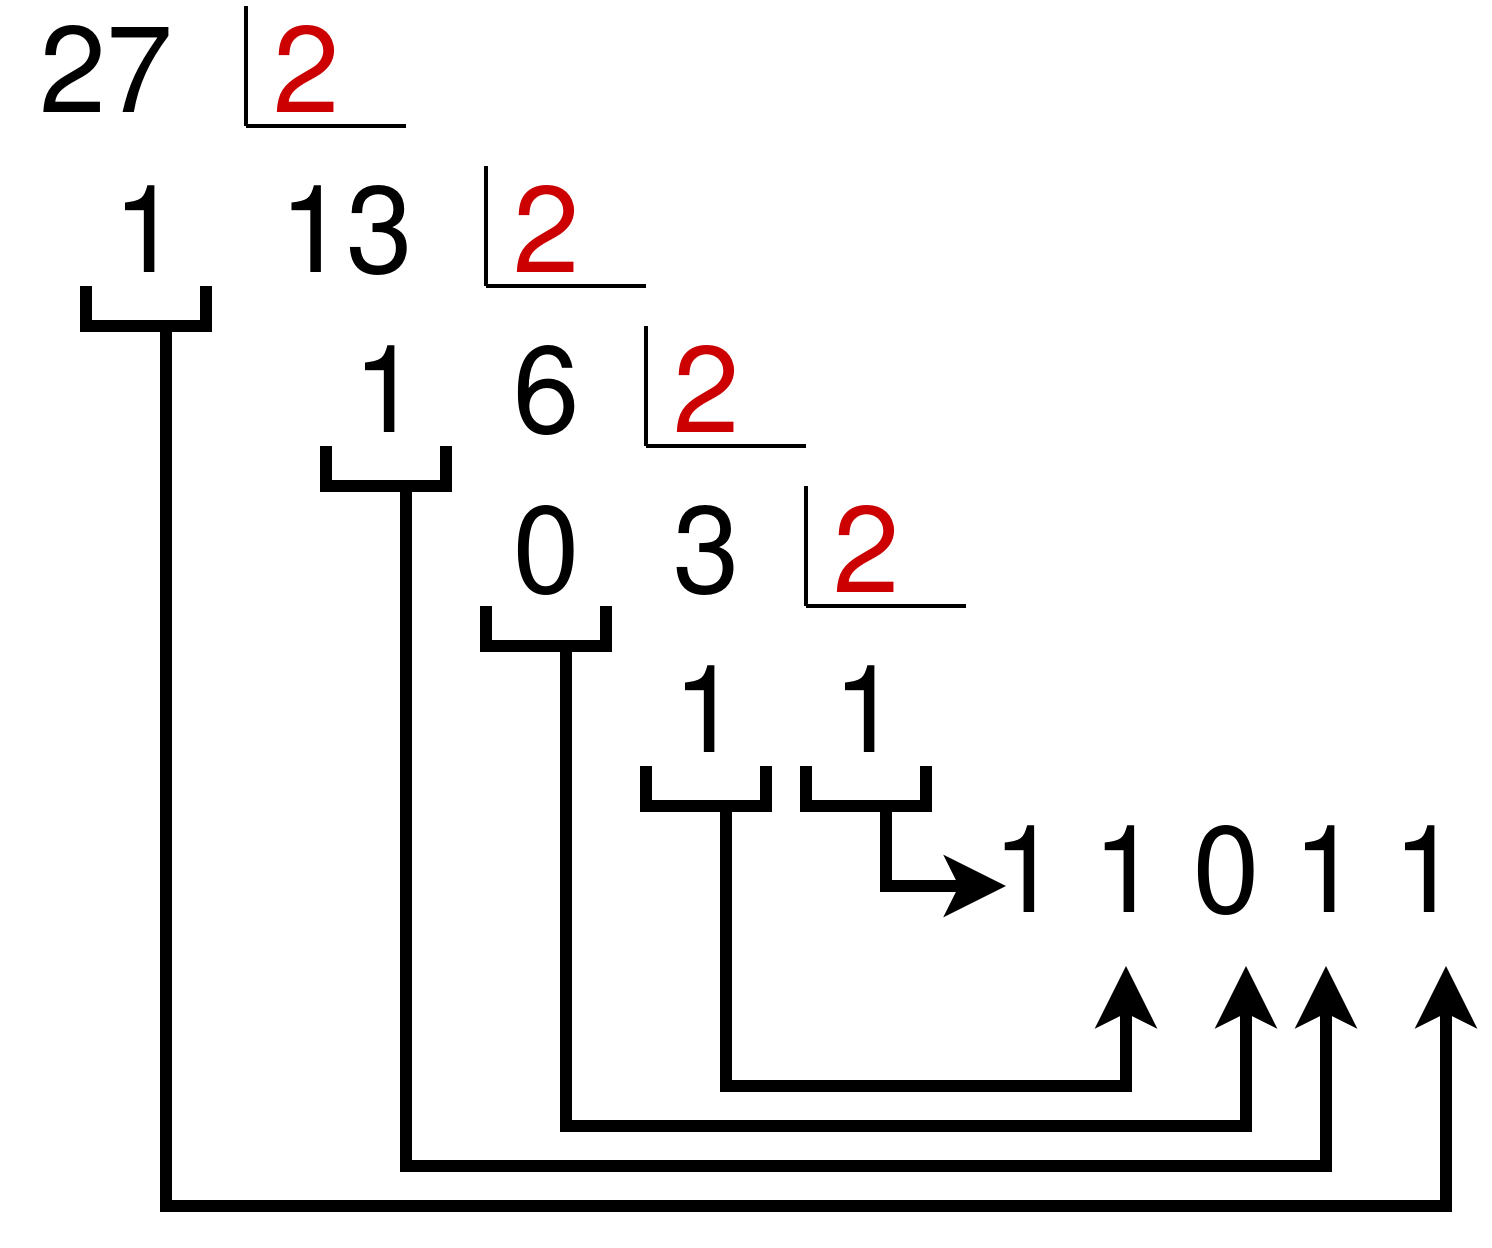
\includegraphics[width=0.29\linewidth]{decimal_binario.png}
    \vspace{-20pt}
\end{center}

\textbf{Los restos los cogemos en orden inverso} para obtener la siguiente equivalencia: $\mathbf{27_{(10} = 11011_{(2}}$

\subsection*{... hexadecimal}
Se trata de dividir sucesivamente el número decimal y los sucesivos cocientes entre 16 (la base hexadecimal). Cuando el cociente o resto sea entre 10 y 15, habrá que cambiarlo por la letra correspondiente.

\begin{center}
    \vspace{-10pt}
    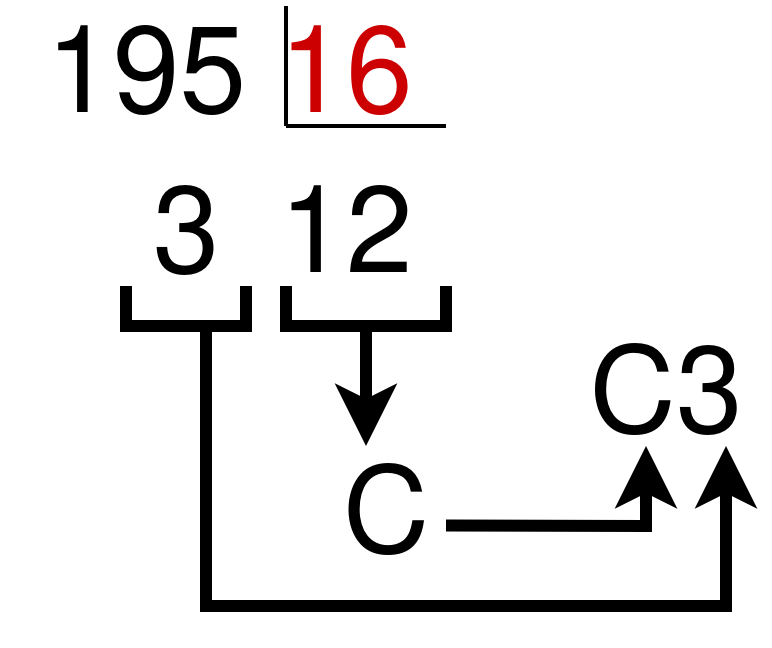
\includegraphics[width=0.2\linewidth]{decimal_hexadecimal.png}
    \vspace{-15pt}
\end{center}

\textbf{Los restos los cogemos en orden inverso} para obtener la siguiente equivalencia: $\mathbf{195_{(10} = C3_{(16}}$

\subsection*{... octal}
Al igual que los anteriores, hacemos divisiones sucesivas:

\begin{center}
    \vspace{-10pt}
    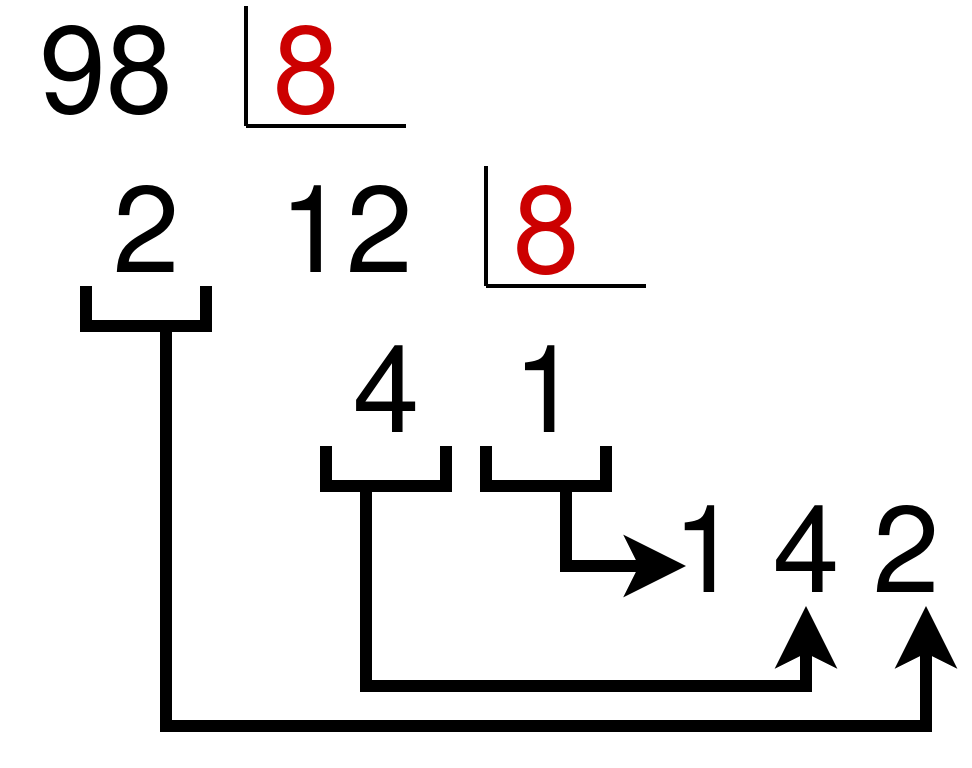
\includegraphics[width=0.25\linewidth]{decimal_octal.png}
    \vspace{-15pt}
\end{center}

\textbf{Los restos los cogemos en orden inverso} para obtener la siguiente equivalencia: $\mathbf{98_{(10} = 142_{(8}}$


\subsection{Conversión de binario a...}

\subsection*{... decimal}
El sistema de numeración binario es un sistema posicional donde cada dígito binario (bit) tiene un valor basado en su posición relativa al \textbf{LSB} (\textit{Least Significant Bit} = bit menos significativo, que es el que está más a la derecha y que tiene el menor valor).

Cualquier número binario puede convertirse a su equivalente decimal multiplicando cada bit por la base (2) y usando como exponente la posición (siendo 0 el exponente del bit de más a la derecha). Para ilustrarlo, cojamos como ejemplo el número binario $\mathbf{11011_{(2}}$:

\begin{center}
    \vspace{-20pt}

    $ \mathbf{11011_{(2}} $

    $ \mathbf{1\times2^4 + 1\times2^3 + 0\times2^2 + 1\times2^1 + 1\times2^0} $

    $ \mathbf{16 + 8 + 0 + 2 + 1 = 27_{(10}} $
    \vspace{-15pt}
\end{center}

Nótese que el procedimiento consiste en determinar los valores (es decir, las potencias de 2) de cada posición de bit que contenga un 1 y luego sumarlos.

Nótese también que el \textbf{MSB} (\textit{Most Significant Bit} = bit más significativo,\textbf{ el que está más a la izquierda}, el que tiene mayor valor) tiene un valor de $\mathbf{2^4}$ a pesar de que es el quinto bit. Esto se debe a que el \textbf{LSB} (\textit{Least Significant Bit}, el bit menos significativo, el que está a la derecha) es el primer bit y tiene un valor de $\mathbf{2^0}$.

\subsection*{... octal}
Para convertir un número binario a octal \textbf{se agrupan los dígitos de 3 en 3 empezando desde el lado derecho} hacia la izquierda, sustituyendo cada trío de dígitos binarios por su equivalente en octal.

Si en el lado izquierdo quedase algún bit “suelto” (sin formar un grupo de 3), se pueden poner “0” a la izquierda.

Cogemos como ejemplo el número binario $\mathbf{1100101001001_{(2}}$ para pasarlo a octal, haremos:

\begin{center}
    \vspace{-15pt}
    $\mathbf{001\ \ 100\ \ 101\ \ 001\ \ 001_{(2} = 14511_{(8}}$
    \vspace{-15pt}
\end{center}

\subsection*{... hexadecimal}
Similar al caso anterior, pero en este caso \textbf{la agrupación que se realiza debe de ser de 4 en 4 bits}. Si usamos el mismo ejemplo anterior $\mathbf{1100101001001_{(2}}$ :

\begin{center}
    \vspace{-15pt}
    $\mathbf{0001\ \ 1001\ \ 0100\ \ 1001_{(2} = 1949_{(16}}$
    \vspace{25pt}
\end{center}



\subsection{Conversión de hexadecimal a...}
\subsection*{... binario}
Para pasar de hexadecimal a binario convertiremos cada símbolo hexadecimal a 4 dígitos binarios.

\begin{center}
    \vspace{-15pt}
    $\mathbf{F17A_{(16} = 1111\ \ 0001\ \ 0111\ \ 1010_{(2}}$

    $\mathbf{1A4F_{(16} = 0001\ \ 1010\ \ 0100\ \ 111_{(2}}$
    \vspace{-15pt}
\end{center}


\subsection*{... decimal}
Al igual que hemos hecho con las conversiones previas a decimal, se podría realizar haciendo potencias de 16, pero se entiende que es más complicado de realizar.

Por lo tanto, \textbf{la manera más sencilla es pasar primero a binario} como acabamos de ver \textbf{y posteriormente convertir ese binario a decimal} como hemos visto previamente.

\subsection*{... octal}
Pasar primero a binario y después a octal.



\subsection{Conversión de octal a...}
\subsection*{... binario}
Cada dígito en octal se convierte en su representación en 3 bits:

\begin{center}
    \vspace{-15pt}
    $\mathbf{167_{(8} = 001\ \ 110\ \ 111_{(2}}$

    $\mathbf{253_{(8} = 010\ \ 101\ \ 011_{(2}}$
    \vspace{-15pt}
\end{center}
Los ceros de la izquierda se podrían quitar, ya que no alteran el valor.

\subsection*{... decimal}
Se puede realizar de dos maneras. La primera es hacer uso de potencias de 8 (similar al paso de pasar de binario a decimal, pero cambiando la base):

\begin{center}
    \vspace{-15pt}
    $\mathbf{157_{(8} = 1\times8^2 + 5\times8^1 + 7\times8^0 = }$

    $\mathbf{1\times64 + 5\times8 + 7\times1 = }$

    $\mathbf{64 + 40 + 7 = 111_{(10}}$

    Resultado: $\mathbf{157_{(8} = 111_{(10}}$
    \vspace{-15pt}
\end{center}

Con números grandes puede ser un poco complicado calcular las potencias de 8, por lo que \textbf{la alternativa es pasarlo primero a binario} como hemos visto, \textbf{y después pasarlo de binario a decimal}.

\subsection*{... hexadecimal}
La manera más sencilla es realizar la conversión primero a binario tal como hemos visto, y posteriormente pasar el número binario a hexadecimal como se ha visto previamente.

\section{Comprobar conversiones}

Podemos hacer uso de la calculadora del sistema Windows para comprobar si estamos realizando de manera correcta las conversiones. El problema es que por defecto sólo hace uso del sistema decimal. Para poder utilizar los sistemas de numeración que hemos aprendido, es necesario utilizar la versión “Programador”.

\begin{center}
    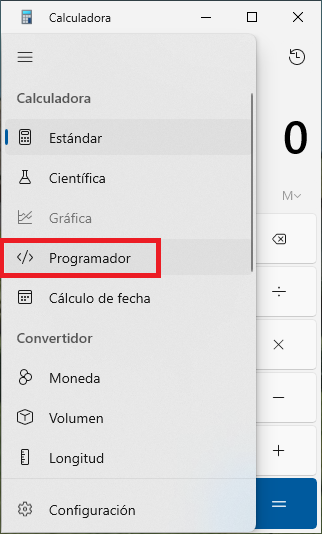
\includegraphics[width=0.45\linewidth]{calculadora1.png}
    \hfill
    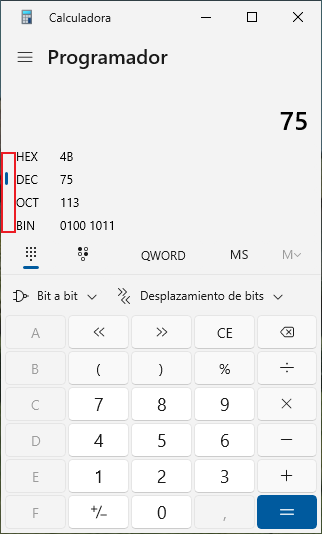
\includegraphics[width=0.45\linewidth]{calculadora2.png}
\end{center}

Una vez está en modo “Programador”, nos debemos fijar qué sistema de numeración está elegido. Al escribir cualquier número, en el resto de opciones veremos las conversiones automáticamente.

    \graphicspath{{../../../temas_comunes/unidades_informacion/img/}}
    \chapter{Unidades de Información digital}

A la hora de almacenar información digital es importante conocer el tamaño del objeto que queremos almacenar y el espacio libre del lugar en el que lo queremos guardar.

En decimal estamos acostumbrados a contar usando el \href{https://es.wikipedia.org/wiki/Sistema_Internacional_de_Unidades}{Sistema Internacional de Unidades}, y dependiendo de la magnitud que queramos medir, haremos uso de unos prefijos establecidos. Por ejemplo, para medir la distancia usamos el \textbf{metro}, y por tanto nos quedaría:

\begin{itemize}
    \item \textbf{Sin prefijo} : metro, una unidad.
    \item \textbf{deca-}metro: $10^1$ metros
    \item \textbf{hecto-}metro: $10^2$ metros
    \item \textbf{kilo-}metro: $10^3$ metros
    \item \textbf{mega-}metro: $10^6$ metros
    \item \textbf{giga-}metro: $10^9$ metros
    \item ...
\end{itemize}

En decimal hacemos uso de la \textbf{base 10}, y por tanto  con cada prefijo lo que estamos haciendo es modificar el exponente que indica la cantidad. Para unidades pequeñas el exponente varía de uno en uno, pero a partir de cierta cantidad (\textbf{kilo-}), la cantidad cambia multiplicando por 1000 ($10^3$).


\section{Sistema binario}

En informática la información se guarda en formato binario, y la unidad más pequeña es el \textbf{bit}, que es un acrónimo de \textit{\textbf{bi}nary digi\textbf{t}}. Cada bit es una única unidad que sólo permite dos estados: \textbf{0} o \textbf{1}. A la hora de representarlo se hace uso de la letra \textbf{b} minúscula, por lo tanto, \textbf{10b} son 10bits.


\subsection{Múltiplos}

Al igual que en decimal, a medida que aumentamos la cantidad, se hace uso de prefijos para facilitar el conocer de qué cantidad estamos hablando.

A continuación se expone una tabla de las medidas más utilizadas:

\begin{yukitblr}{X X X}
    Nombre & Símbolo & Cantidad \\
    \textbf{Bit} & \textbf{b} & $2^0=1$ \\
    Nibble & & 4b \\
    \textbf{Byte} & \textbf{B} & 8b \\
    \textbf{Kibi}byte & \textbf{KiB} & $2^{10}=1024 B$ \\
    \textbf{Mebi}byte & \textbf{MiB} & $2^{20}=1024 KiB$ \\
    \textbf{Gibi}byte & \textbf{GiB} & $2^{30}=1024 MiB$ \\
    \textbf{Tebi}byte & \textbf{TiB} & $2^{40}=1024 GiB$ \\
    \textbf{Pebi}byte & \textbf{PiB} & $2^{50}=1024 TiB$ \\
    \textbf{Exbi}byte & \textbf{EiB} & $2^{60}=1024 PiB$ \\
\end{yukitblr}

Aunque esta es la manera correcta de nombrar las unidades cuando hablamos en términos informáticos, lo habitual es que se haga uso de los prefijos del sistema decimal.

\section{Usos}

A la hora de utilizar las medidas vistas previamente hay que diferenciar qué queremos medir, ya que no se hará siempre igual.

\begin{itemize}
    \item \textbf{Almacenamiento}: A la hora de querer expresar una cantidad de almacenamiento (para un disco duro, un \textit{pendrive} USB, RAM, ...) se hace uso del \textbf{Byte} y de sus múltiplos usando los prefijos vistos previamente.

    \begin{center}
        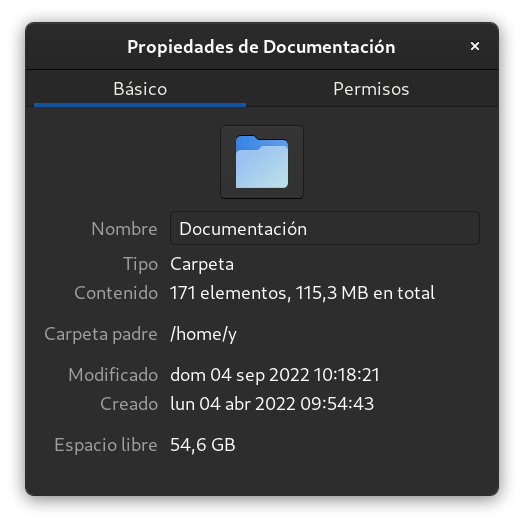
\includegraphics[width=0.4\linewidth]{hdd.png}
    \end{center}

    \item \textbf{Transmisión}: Cuando hablamos de tasa de transferencia de datos se hace uso del término “tasa de bits” (en inglés \textit{\textbf{bitrate}}), que indican el número de bits que se transmiten por unidad de tiempo. Hoy día se suele medir en kbps (o kb/s, kilobits por segundo), Mbps (Mb/s, o megabit por segundo), ... Para convertirlo a Bytes por segundo habría que dividirlo por “8”.

    \begin{center}
        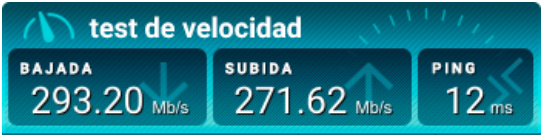
\includegraphics[width=0.4\linewidth]{bitrate.png}
    \end{center}

\end{itemize}

\warnbox{\textbf{La transmisión de datos se expresa en “bits por segundo”}}

    \vfill
    \pagebreak
    \part{GNU/Linux}
    \graphicspath{{../../../temas_comunes/gnu_linux/img}}
    \chapter{Introducción a GNU/Linux}
\section{Un poco de historia}
Para conocer cómo nació el movimiento GNU y el kernel Linux debemos conocer un poco de historia de la informática y cómo evolucionó en los primeros años.

\subsection{El nacimiento de Unix}

\begin{description}
\item[1964-1969]Los laboratorios \textbf{Bell} empiezan un proyecto con el \textbf{MIT} (Instituto Tecnológico de Massachusetts) y \textbf{General Electric} para desarrollar un sistema de \textbf{tiempo compartido} (“time-sharing computing”): se llamaría \textbf{Multics} (Multiplexed Information and Computing Service).

Hasta este momento, los sistemas utilizados eran de un único proceso, la CPU no era compartida por múltiples procesos sino que se ejecutaba por lotes (se les mandaba los procesos a ejecutar y se ejecutaban en orden).

Multics obtuvo licencia libre en el 2007. En Diciembre del 2016 salió la última versión 12.6f.

\itemimage{1969}{r}{0.33}
  {/Ken_Thompson_and_Dennis_Ritchie--1973.jpg}
  {\href{https://en.wikipedia.org/wiki/Ken_Thompson}{Ken y Dennis. Origen: Wikipedia}}
  {
  Uno de los desarrolladores de Multics, \href{https://en.wikipedia.org/wiki/Ken_Thompson}{Ken Thompson}, decidió escribir su propio sistema operativo. Ken Thompson es conocido también por crear el lenguaje de programación \textbf{B}, el sistema de codificación de caracteres UTF-8 y el lenguaje de programación Go, entre otras cosas.

A Ken Thompson se le une \href{https://en.wikipedia.org/wiki/Dennis_Ritchie}{Dennis Ritchie} y otros, y empiezan a programar un sistema de ficheros jerárquico, el concepto de procesos de computación, ficheros de dispositivos, un intérprete de comandos, … El resultado de lo programado era más pequeño y simple que Multics, lo que se convertiría en Unix. En Agosto ya tendrían el sistema operativo, se auto-gestiona,  tenía un assembler, un editor y una shell de comandos.

Dennis Ritchie es conocido también por crear junto con Ken el lenguaje de programación \textbf{C} (aparece por primera vez en 1972).
}


\item[1970]En ese momento el nuevo sistema operativo se llamaba \textbf{Unics} (\textit{Uniplexed Information and Computing Service}, un juego de palabras en contraposición a  Multics). No tenían todavía dinero de la organización en el desarrollo (era desarrollado por los programadores) y tampoco era multitarea todavía.

A finales de año el sistema ya era conocido como \textbf{UNIX}, y se había portado a la máquina PDP-11.

\textbf{Las primeras versiones de Unix incluían el código fuente} para que las universidades lo pudiesen modificar y así poder extenderlo a sus necesida des.


\item[1971]El sistema se empieza a hacer complejo y como querían que más usuarios lo usasen, crean el sistema de manuales que es utilizado hoy en día (mediante el comando \textbf{"man"}).

\begin{center}
  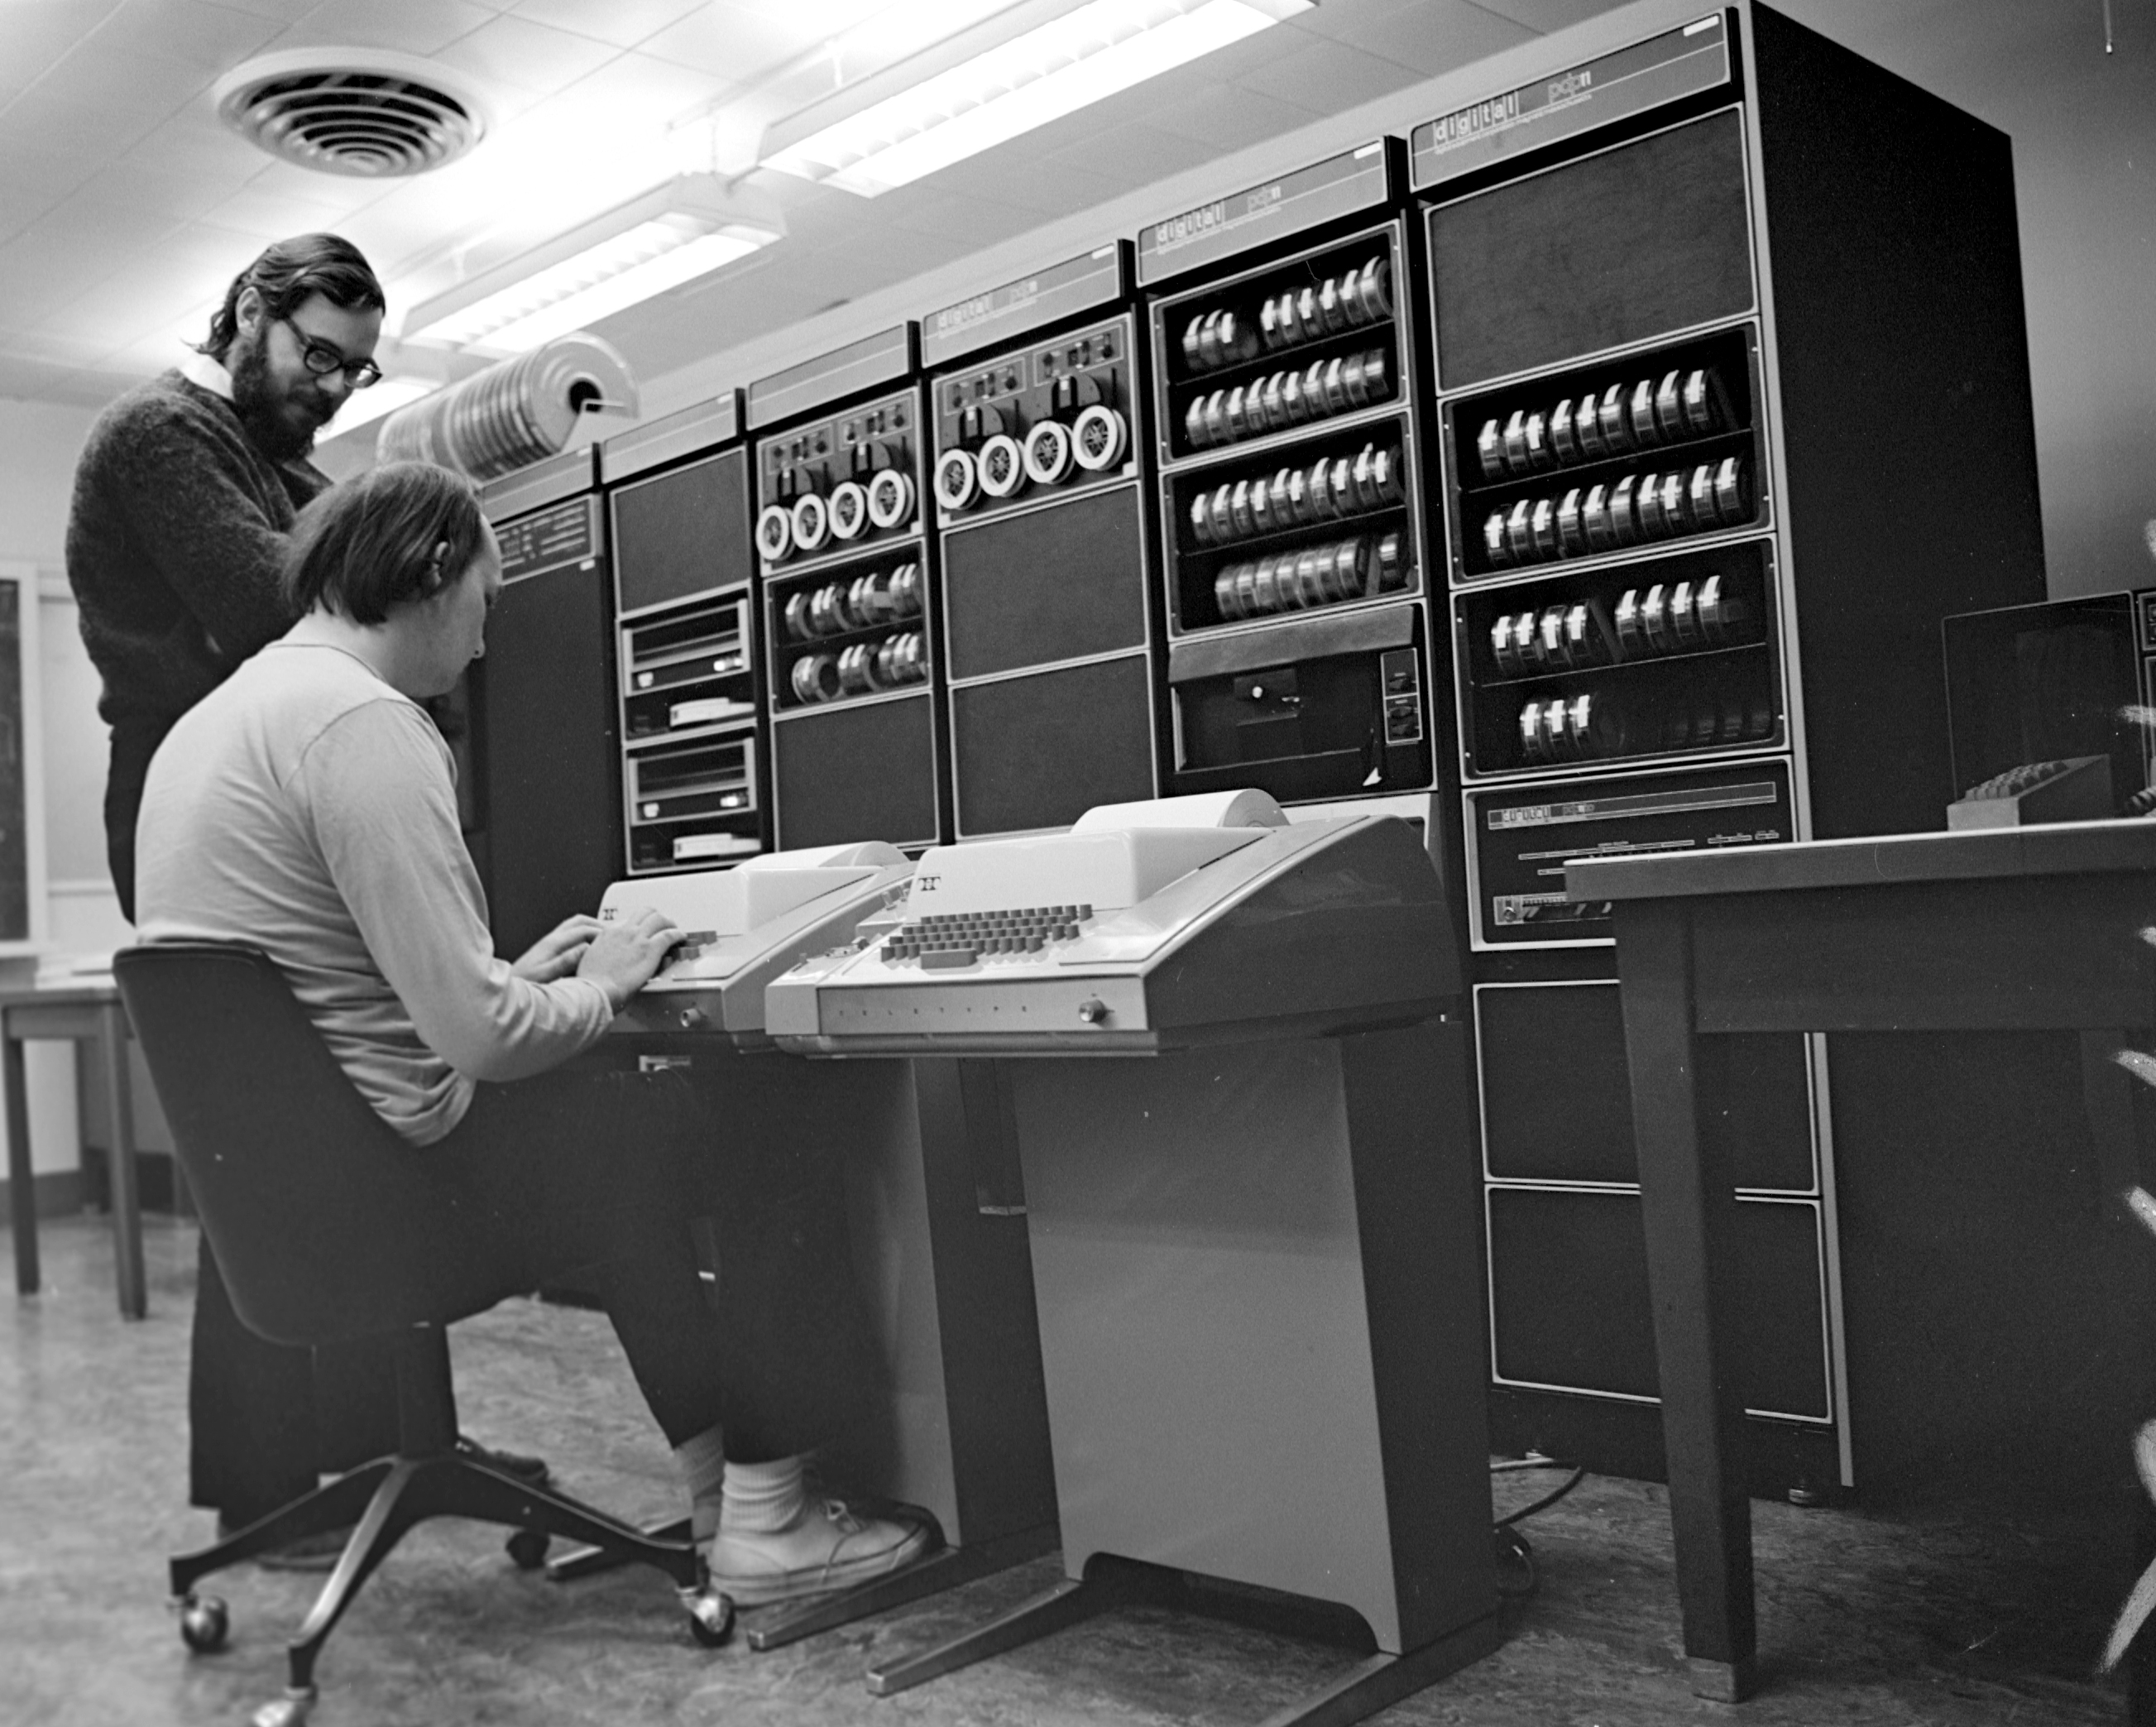
\includegraphics[width=0.8\linewidth]{/Ken_Thompson_(sitting)_and_Dennis_Ritchie_at_PDP-11_(2876612463).jpg}
  \vspace{-10pt}\captionof{figure}{\href{https://en.wikipedia.org/wiki/Ken_Thompson}{Dennis Ritchie y Ken Thompson trabajando en un PDP-11. Origen: Wikipedia}}\vspace{-13pt}
\end{center}


\item[1973]La versión 4 del sistema es reescrita completamente en C. Hasta este momento el sistema había estado escrito en ensamblador, por lo que no era portable entre distintos tipos de máquinas, aunque la primera versión portada a otra plataforma fue en 1978. Se cree que había “más de 20” instalaciones del sistema.

\item[1974]La versión 5 se licencia para ser utilizada en \textbf{instituciones educativas}.

\item[1975]La versión 6 se licencia para poder ser utilizadas por empresas por \$20.000 de la época.

\item[1977]La universidad de Berkeley lanza su primera versión de Unix bajo la Berkeley Software Distribution (BSD).

\item[1979]Con la salida de Unix v7, se comienza a portar a los distintos ``microordenadores'' de la época y a los distintos microprocesadores (Motorola 68000, Intel 8086, … ).

\item[1980]Microsoft anuncia su primer Unix para microcomputadoras de 16 bits (Xenix).
\end{description}

\subsection{El nacimiento de GNU (GNU's Not Unix)}
\begin{description}

\item[1971]\href{https://en.wikipedia.org/wiki/Richard_Stallman}{Richard Stallman} comienza su carrera en el MIT en el laboratorio de inteligencia artificial.

Es conocido no sólo por el movimiento GNU, si no también por crear GCC y Emacs entre otra gran cantidad de software.

En esa época el software se distribuía de manera abierta para poder ser modificado. Lo habitual era realizar modificaciones para mejorar el software y distribuirlo entre compañeros y universidades.

\itemimage{1982}{r}{0.25}
  {/Richard_Stallman_2016_Talk_in_Madrid_06.jpg}
  {\href{https://commons.wikimedia.org/wiki/File:Richard_Stallman_2016_Talk_in_Madrid_06.jpg}{Richard Stallman: Wikimedia}}
  {
Richard Stallman quiere modificar el firmware de unas impresoras y el fabricante le pide que firme un acuerdo de no divulgación si le enseñan el código. Esto hace que Stallman se enfurezca y es cuando decide que la situación actual debe cambiar y volver al sistema de intercambio de software anterior.

\item[1983] Se anuncia el nacimiento del proyecto \textbf{GNU}, cuya finalidad es la de construir un sistema operativo completamente libre, compatible con Unix. La idea es dar a los usuarios la libertad y el control de sus ordenadores.

\item[1985] Se lanza el \href{https://www.gnu.org/gnu/manifesto.es.html}{manifiesto GNU}, y ya cuenta con un editor de texto (Emacs), compilador de C, una shell, varias utilidades … El núcleo inicial todavía no es funcional.
}


\item[1986]
Richard Stallman escribe y publica la definición de lo que es Free Software (Software Libre) a través de la \href{https://es.wikipedia.org/wiki/Free_Software_Foundation}{Free Software Foundation}.

\begin{tcolorbox}[title=Aclarando la palabra “free”:,sidebyside,righthand width=0.12\linewidth]

\textbf{The word “free” in our name does not refer to price; it refers to freedom.}

La palabra “free” no se refiere a gratis, si no que se refiere a libertad.

\tcblower

\includegraphics[width=\linewidth]{/gnu.png}
\end{tcolorbox}

Más adelante veremos a qué se refiere sobre libertad en el software.

\end{description}

\subsection{El nacimiento de Minix}
\begin{description}
\item[1987]Andrew S. Tanenbaum crea  Minix como propósito educativo y para enseñar cómo funciona un sistema operativo.

\item[1991]Sale la versión 1.5 de Minix y es portada a distintas arquitecturas (IBM, Motorola 68000, Amiga, Apple Macintosh, …).

\item[1992]Debate con Linus Torvalds sobre la arquitectura del kernel Linux (núcleo monolítico) en lugar de usar un micronúcleo.

\end{description}


\subsection{El nacimiento de Linux}
\begin{description}

\item[1991] Un estudiante en la universidad de Helsinki, \href{https://en.wikipedia.org/wiki/Linus_Torvalds}{Linus Torvalds}, comienza un proyecto personal escrito para su nuevo ordenador, un PC con procesador 80386.

El desarrollo comienza bajo \textbf{Minix}, usando el compilador \textbf{GCC} del movimiento GNU (GCC = GNU Compiler Collection).

El proyecto termina convirtiéndose en un kernel de un sistema operativo y escribió al grupo de noticias de Minix diciendo:

\begin{tcolorbox}[title=Email de Linus Torvalds presentando Linux,sidebyside,righthand width=0.30\linewidth]
  “Hola a todos los que estáis ahí fuera usando minix.\\


  Estoy haciendo un sistema operativo (libre), (solamente por aficion, no será grande ni profesional como el GNU) para clones 386(486) AT.

  ...

  PD. Sí – está libre de cualquier código de minix, y tiene un sistema de ficheros multi-hilo. NO es portable (usa el cambio de tareas del 386 etc), y probablemente nunca soporte otra cosa que no sean los discos duros AT, porque es todo lo que tengo :-(. ”
  \tcblower
  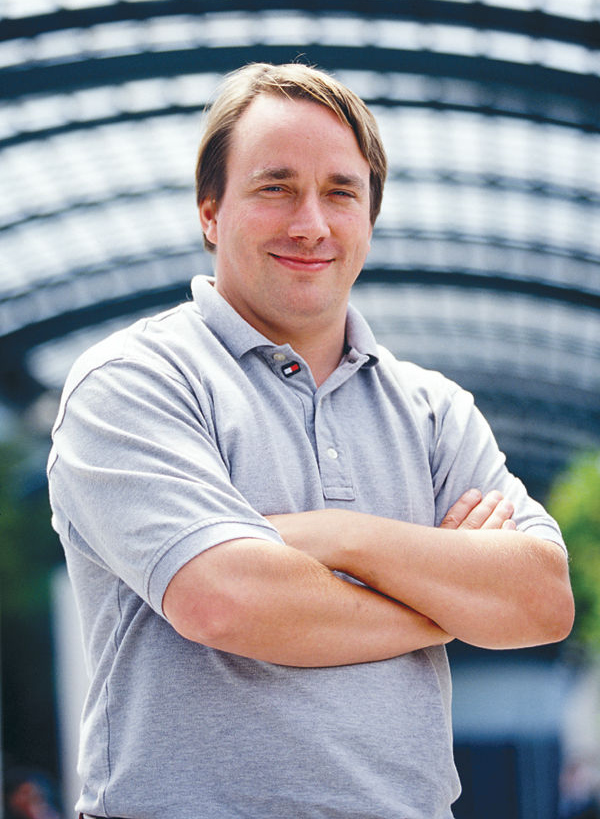
\includegraphics[width=\linewidth]{/Linus_Torvalds.jpeg}
  \vspace{-30pt}\captionof{figure}{\href{https://en.wikipedia.org/wiki/Linus_Torvalds}{Linus torvalds. Origen: Wikipedia}}
\end{tcolorbox}


\item[1992] Originalmente la licencia de Linux era propia e impedía el uso comercial de Linux. En la versión 0.99 esto cambia y se cambia a la licencia GNU Public License (\textbf{GPL}).

\item[1993] El proyecto cuenta con más de 100 desarrolladores. El kernel se adapta al entorno del proyecto GNU. Nace la distribución \textbf{Debian} (una de las más importantes a día de hoy)

\begin{center}
  
\includegraphics[width=0.5\linewidth]{/debian-logo.jpg}
  \vspace{-10pt}\captionof{figure}{\href{https://www.debian.org}{Debian}}
\end{center}

\item[1994] Se libera la versión 1.0. El proyecto XFree86 se une y Linux consigue interfaz gráfico. Nacen las primeras distribuciones comerciales \textbf{Red Hat} y \textbf{Suse}.

\item[1998] Empresas como \textbf{IBM}, \textbf{Compaq} y \textbf{Oracle} anuncian que apoyan a Linux. Nace el interfaz gráfico \textbf{KDE}.

\item[1999] Nace el interfaz gráfico \textbf{GNOME} como reemplazo a KDE, ya que KDE hacía uso de una librería propietaria en aquel momento (QT).

\item[2001] Steve Ballmer (CEO de Microsoft) dice: \textbf{“Linux es un cáncer”}.

\item[2002] Se libera OpenOffice (originalmente suite ofimática de Sun Microsystems). Nace Mozilla (hoy día:  Firefox).

\item[2003] IBM lanza un anuncio para la Linux Foundation: \href{https://www.youtube.com/watch?v=x7ozaFbqg00}{https://www.youtube.com/watch?v=x7ozaFbqg00}

\item[2004] Nace \textbf{Ubuntu} (basándose en Debian) y Steve Ballmer (CEO de Microsoft) dice que Linux infringe muchas de sus patentes.

\item[2008] Nace \textbf{\href{https://es.wikipedia.org/wiki/Android}{Android}}, sistema operativo con kernel Linux. Actualmente es el sistema operativo de móviles que más terminales tiene.

\item[2009] Red Hat iguala a Sun Microsystem en capitalización bursátil (un gran logro simbólico).

\item[2014] Satya Nadella (CEO de Microsoft) muestra en una presentación la siguiente transparencia:

\begin{center}
  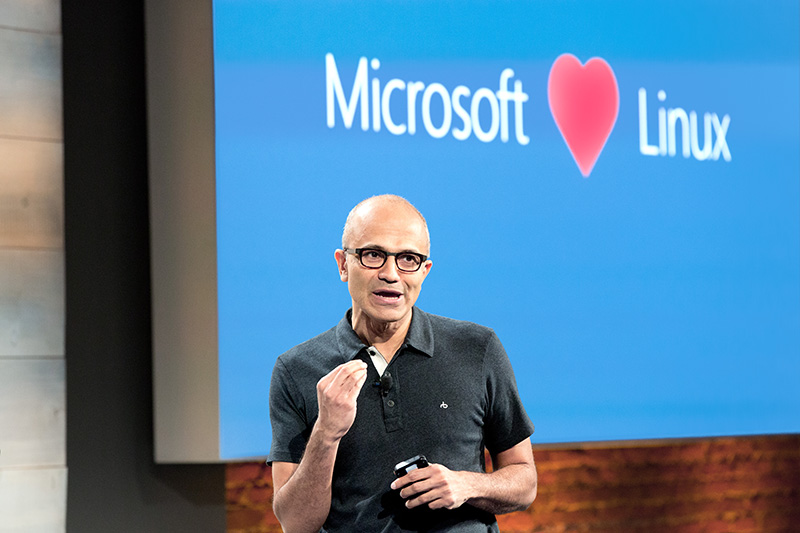
\includegraphics[width=0.5\linewidth]{/Microsoft_Linux.jpg}
  \vspace{-10pt}\captionof{figure}{\href{https://commons.wikimedia.org/wiki/File:Microsoft_Linux.jpg}{Origen: Wikipedia}}
\end{center}


\item[2016]
Microsoft anuncia \href{https://es.wikipedia.org/wiki/Windows_Subsystem_for_Linux}{WSL} (\textit{Windows Subsystem for Linux}) y se puede instalar en Windows 10 y Windows Server 2019. Permite correr ejecutables de Linux nativamente.

\end{description}

\subsection{Cronograma de sistemas Unix}
En el siguiente cronograma se puede ver la línea temporal de los sistemas Unix:

\begin{center}
  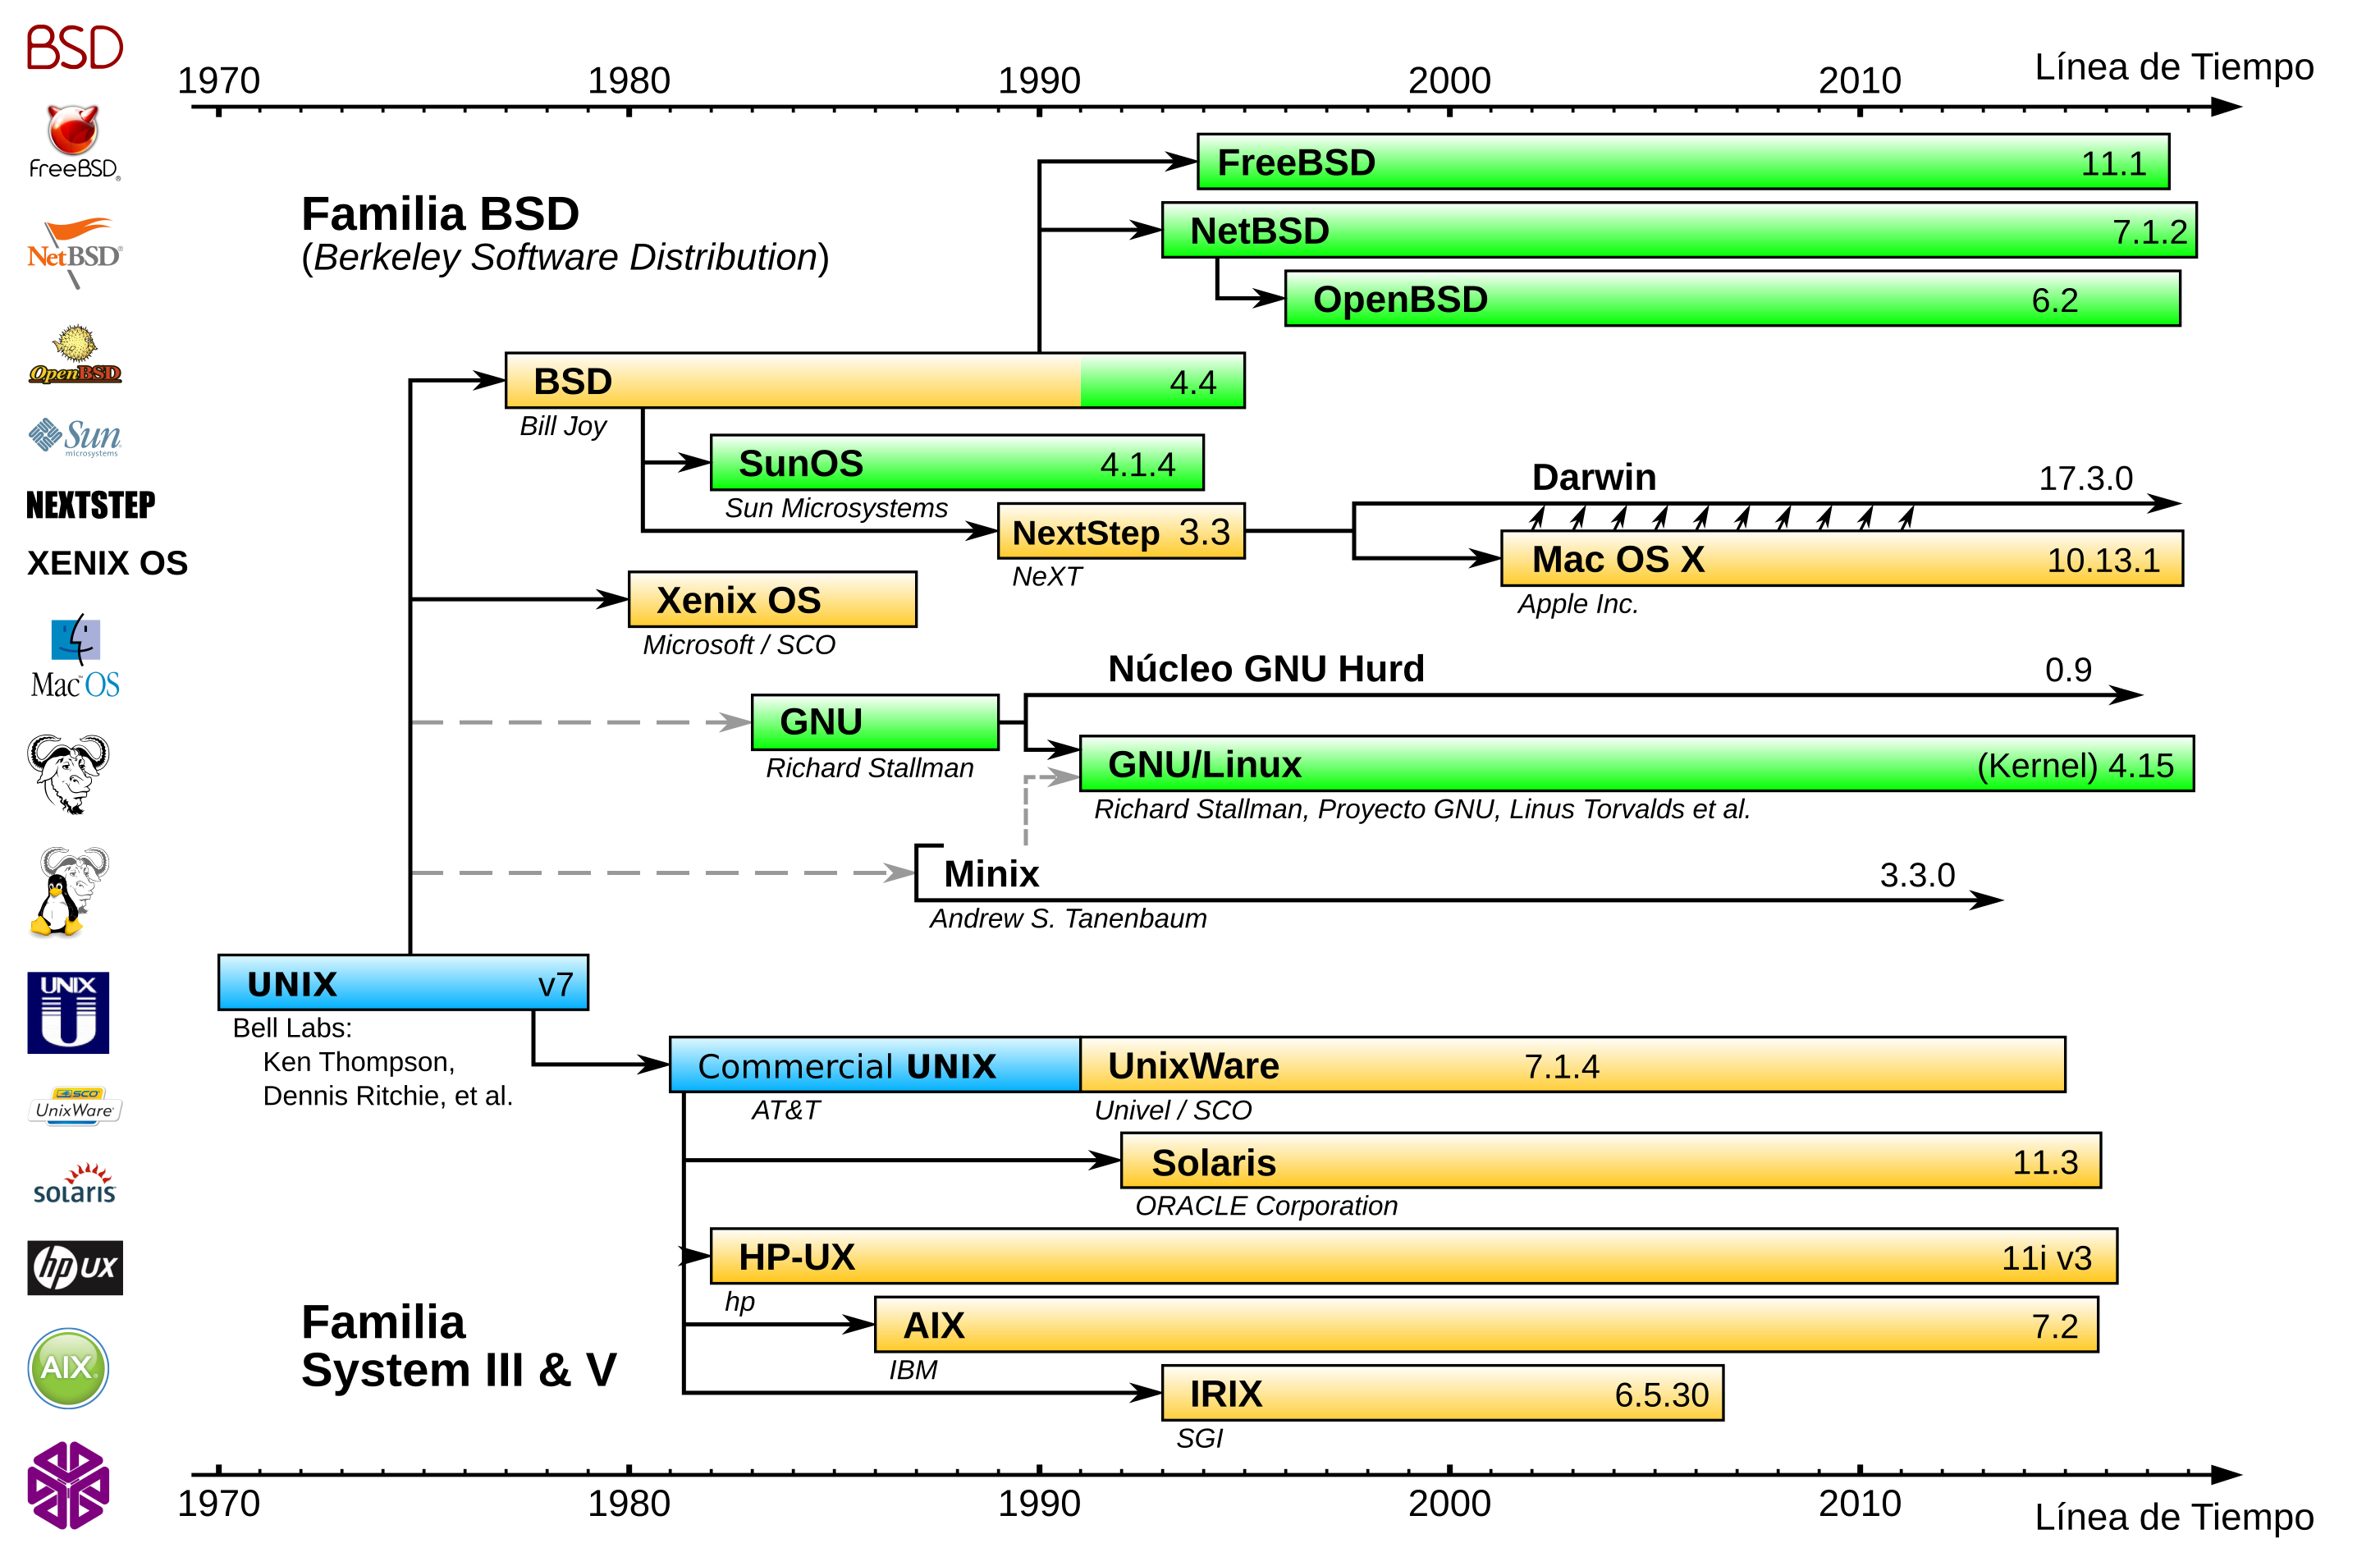
\includegraphics[width=0.7\linewidth]{/Evolución_UNIX.png}
  \vspace{-10pt}\captionof{figure}{\href{https://commons.wikimedia.org/wiki/File:Evolución_UNIX.png}{Origen: Wikipedia}}
\end{center}

\section{Resumen}
Linux es conocido como un sistema operativo libre pero el nombre de Linux se  centra única y exclusivamente en el \textbf{kernel} (o \textbf{núcleo}) del sistema operativo.

El sistema operativo completo debería llamarse \textbf{GNU/Linux}, ya que el kernel es una “pequeña” parte (aunque muy importante) dentro de todo el sistema operativo. El resto de herramientas utilizadas en el sistema operativo pertenecen al proyecto GNU.


\chapter{Licencias Libres}
%<*softwarelibre>
\section{Free Software / Software Libre}

En 1986 Richard Stallman saca a la luz la definición de lo que es Free Software (Software Libre) a través de la \href{https://es.wikipedia.org/wiki/Free_Software_Foundation}{Free Software Foundation}:

\begin{tcolorbox}[title=Aclarando la palabra “free”:,sidebyside,lower separated=false,righthand width=0.12\linewidth]

    \textbf{The word “free” in our name does not refer to price; it refers to freedom.} \linebreak

    La palabra “free” no se refiere a gratis, se refiere a \textbf{libertad}.

    \tcblower
    
\includegraphics[width=\linewidth]{/gnu.png}
\end{tcolorbox}


Las libertad en el software se refiere a:
\begin{tcolorbox}[title=Libertades del Software Libre:]
    \begin{enumerate}
        \setcounter{enumi}{-1}
        \item La libertad de ejecutar el programa, para cualquier propósito .

        \item La libertad de estudiar cómo trabaja el programa, y cambiarlo para que haga lo que usted quiera. El acceso al código fuente es una condición necesaria para ello.

        \item La libertad de redistribuir copias para que pueda ayudar al prójimo.

        \item La libertad de mejorar el programa y publicar sus mejoras, y versiones modificadas en general, para que se beneficie toda la comunidad. El acceso al código fuente es una condición necesaria.
    \end{enumerate}
\end{tcolorbox}

El movimiento del Free Software es un movimiento que tiene que ver más con la filosofía y la ética que con la tecnología en sí misma.


\subsection{Copyleft y GNU Public License (GPL)}
Es una práctica legal que consiste en el ejercicio del derecho de autor (copyright en inglés) con el objetivo de propiciar el libre uso y distribución de una obra, exigiendo que los concesionarios preserven las mismas libertades al distribuir sus copias y derivados (\href{https://es.wikipedia.org/wiki/Copyleft}{Wikipedia}).

\begin{center}
  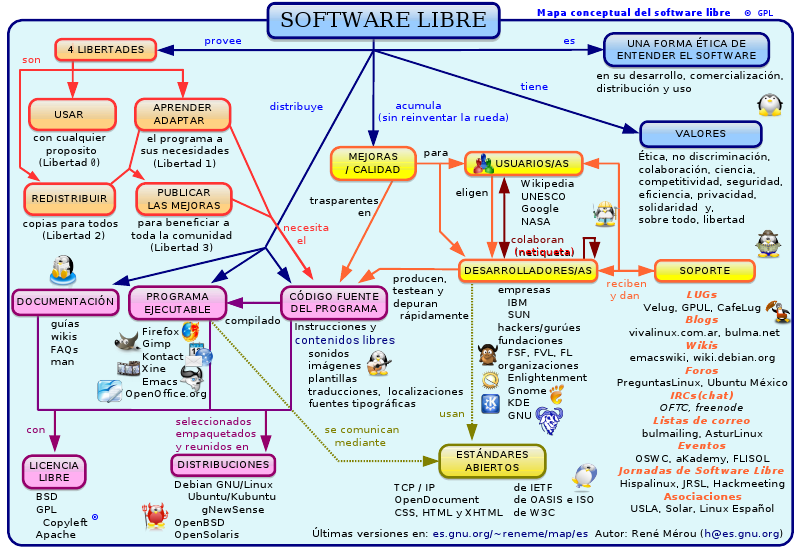
\includegraphics[width=\linewidth]{Mapa_conceptual_del_software_libre.png}
  \vspace{-30pt}\captionof{figure}{\href{https://commons.wikimedia.org/wiki/File:Mapa_conceptual_del_software_libre.png}{Mapa conceptual del Software Libre: Wikipedia}}\vspace{-20pt}
\end{center}

Con esto nació la licencia GNU GPL, la cual permite al usuario final la libertad de usar, estudiar, compartir y modificar el software recibido. Tiene que quedar claro que un programa comercial puede ser Software Libre.

\subsection{Diferencias con el Open Source}
Los programas Open Source son aquellos que podemos ver el código fuente pero esto no quiere decir que podamos modificarlo o adaptarlo a nuestras necesidades.

El Open Source es menos restrictivo que el Software Libre y se puede decir que todo Software Libre es Open Source, pero no todo Open Source tiene por qué ser libre.


\subsection{Licencias libres más conocidas}
Un listado de las licencias libres más utilizadas (en la \href{https://es.wikipedia.org/wiki/Anexo:Comparaci\%C3\%B3n_de_licencias_de_software_libre}{Wikipedia} existe una tabla comparativa):

\begin{itemize}
    \item \href{https://es.wikipedia.org/wiki/GNU_General_Public_License}{GNU GPL}
    \item \href{https://es.wikipedia.org/wiki/Licencia_BSD}{BSD}
    \item \href{https://es.wikipedia.org/wiki/Licencia_MIT}{MIT}
    \item \href{https://es.wikipedia.org/wiki/Apache_License}{Licencia Apache}
    \item \href{https://es.wikipedia.org/wiki/Licencia_PHP}{Licencia PHP}
    \item \href{https://es.wikipedia.org/wiki/Licencias_Creative_Commons}{Creative Commons} (no todas las versiones). Más utilizadas en contenido multimedia.
\end{itemize}
%</softwarelibre>

\chapter{Sistema de ficheros en GNU/Linux}
El sistema de ficheros en GNU/Linux, al igual que en Unix, es jerárquico, comenzando en la raíz denominada “/”. Partiendo de esta raíz, el resto del sistema de ficheros nace en forma de ramificaciones generando lo que se denominan “rutas de ficheros”, que es el camino completo para llegar al mismo.

\section{Filesystem Hierarchy Standard}
Debido a que en GNU/Linux todo se representa como ficheros (discos, dispositivos, programas, … ) es necesario que exista un orden a la hora de ser almacenados. Con esa intención nace en 1993 el estándar de la jerarquía de ficheros de Linux, enfocado a reestructurar los archivos. Posteriormente se unieron otros derivados de UNIX (la comunidad de desarrollo de BSD) por lo que terminó adoptando el nombre FHS.

Aún siendo un estándar, no todas las distribuciones lo siguen al pie de la letra, y otros Unix, como MacOS, tienen sus propias rutas especiales.


\section{Directorios importantes}
A continuación se exponen los directorios más importantes del sistema junto con la descripción del contenido que deben de tener:
\begin{itemize}

    \item \textbf{/boot/}: archivos de arranque del kernel, normalmente junto con la configuración utilizada para compilarlos.
    \item \textbf{/dev/}: contiene archivos especiales de bloque que representan los dispositivos del hardware que está corriendo el sistema operativo
    \item \textbf{/etc/}: contiene los archivos de configuración del servidor y de los servicios que corren en él. Está subdividido en directorios por servicios o configuraciones.
    \item \textbf{/home/}: los directorios de trabajo de los usuarios normales del sistema
    \item \textbf{/lib/}: librerías que hacen funcionar a los programas
    \item \textbf{/root/}: es la home del usuario root
    \item \textbf{/var/}: archivos variables del sistema
    \begin{itemize}
      \item \textbf{/var/lib/}: aquí se suelen guardar los ficheros de los programas que “crecen”: bases de datos, ficheros caché…
      \item \textbf{/var/log/}: los logs del sistema
    \end{itemize}
\end{itemize}

Junto a todos estos directorios, se ha separado los lugares en los que van los binarios, o ejecutables de los programas. Lo habitual es que se encuentren en estas rutas:

\begin{itemize}
    \item \textbf{/bin/}: aplicaciones esenciales del sistema
    \item \textbf{/sbin/}: aplicaciones que en principio sólo debería ejecutar el usuario root o programas de administración del sistema
    \item \textbf{/usr/bin/}: ejecutables de usuario
    \item \textbf{/usr/sbin/}: ejecutables de superusuario
\end{itemize}
Aunque las rutas de los ejecutables denotan quién debería ejecutar el programa, en la vida real no tiene por qué ser una limitación.

\section{Dispositivos de almacenamiento y discos duros}
En sistemas operativos Windows es habitual que cada partición cuente con una letra para acceder a ella, al igual que ocurre cuando introducimos un dispositivo de almacenamiento externo (un pendrive).

Tal como se ha comentado, en sistemas Unix el sistema de ficheros es una jerarquía, y por tanto todo dispositivo de almacenamiento nuevo deberá estar montado bajo la raíz “/”. Hoy día, en distribuciones con escritorio, al introducir un pendrive éste es auto-montado (es accesible) desde la ruta \textbf{/media/}, donde aparecerán tantos directorios como discos hayamos conectado.

\subsection{Almacenamiento permanente}
Si queremos que un disco duro nuevo sea permanente en nuestro sistema, podremos montarlo en cualquier lugar de la estructura jerárquica. Debido a este sistema, el usuario final no se tendrá que preocupar en almacenar los ficheros en una ruta distinta, si no que será el administrador el que haya hecho que esa ruta ahora pertenezca a un disco duro nuevo.

Imaginemos que el sistema operativo se ha instalado en un disco duro pequeño de 32Gb de espacio y se está llenando, y el directorio que más ocupa es el directorio de los usuarios. Podremos añadir al servidor un nuevo disco duro montado en /home y por tanto a partir de ahora los datos guardados en /home estarán en un nuevo disco duro más grande.

\begin{mycode}{Ejemplo de discos en un sistema con ``lsblk''`}{console}{}
root@vega:~# lsblk
NAME                       MAJ:MIN RM   SIZE RO TYPE MOUNTPOINTS
sda                          8:0    0   1,8T  0 disk
└─sda1                       8:1    0   1,8T  0 part /home/backup

sdb                          8:16   0   3,6T  0 disk
└─sdb1                       8:17   0   3,6T  0 part /home/disco4tb
sdc                          8:32   0 447,1G  0 disk
├─sdc1                       8:33   0   529M  0 part
├─sdc2                       8:34   0   100M  0 part
├─sdc3                       8:35   0    16M  0 part
└─sdc4                       8:36   0 446,5G  0 part
nvme0n1                    259:0    0 931,5G  0 disk
├─nvme0n1p1                259:1    0   512M  0 part
└─nvme0n1p2                259:2    0   800G  0 part /home
nvme1n1                    259:3    0 931,5G  0 disk
├─nvme1n1p1                259:4    0   512M  0 part /boot/efi
├─nvme1n1p2                259:5    0    90G  0 part /
├─nvme1n1p3                259:6    0   300G  0 part
│ ├─VMs-ubuntu--20.04--so1 254:0    0    10G  0 lvm
│ ├─VMs-manjaro            254:2    0    20G  0 lvm
│ └─VMs-win10              254:3    0    35G  0 lvm
└─nvme1n1p4                259:7    0 156,2G  0 part
\end{mycode}


\chapter{Gestión de usuarios locales en GNU/Linux}
En las distribuciones GNU/Linux lo habitual suele ser que existan al menos dos usuarios tras una instalación:

\begin{itemize}
    \item \textbf{root}: usuario administrador o súper usuario.
    \item \textbf{usuario no-privilegiado}: durante la instalación de la distribución nos suele preguntar para crear un usuario del sistema, que no tendrá privilegios.
\end{itemize}


El usuario root, como se ha dicho previamente, es el administrador del sistema, tiene permisos para realizar cualquier tarea dentro de nuestro sistema: instalar paquetes, desinstalarlos, modificar cualquier fichero, realizar formateos... Por lo tanto, el \textbf{realizar tareas como usuario root puede ser peligroso si cometemos algún fallo}.

Las buenas prácticas nos dicen que las tareas cotidianas del sistema deberíamos realizarlas como usuario normal y \textbf{sólo convertirnos en root cuando sea estrictamente necesario}.

\section{Creación de usuarios locales}

Tras instalar el sistema, veremos que se nos han creado varios usuarios en el sistema, aparte del usuario \textbf{root} y el usuario \textbf{no-privilegiado}. Para poder ver los usuarios que existen en nuestro sistema podemos verlo en el fichero \configfile{/etc/passwd} o podríamos obtener un listado ejecutando el siguiente comando:


\begin{mycode}{Listar usuarios del sistema}{console}{}
root@vega:~# cut -d: -f1 /etc/passwd
\end{mycode}

Para crear un usuario:

\begin{mycode}{Crear usuarios del sistema}{console}{\small}
root@vega:~# adduser ruben

Añadiendo el usuario `ruben' ...
Añadiendo el nuevo grupo `ruben' (1001) ...
Añadiendo el nuevo usuario `ruben' (1001) con grupo `ruben' ...
Creando el directorio personal `/home/ruben' ...
Copiando los ficheros desde `/etc/skel' ...
Nueva contraseña:
Vuelva a escribir la nueva contraseña:
passwd: contraseña actualizada correctamente
Cambiando la información de usuario para ruben
Introduzca el nuevo valor, o pulse INTRO para usar el valor predeterminado
    Nombre completo []:
    Número de habitación []:
    Teléfono del trabajo []:
    Teléfono de casa []:
    Otro []:
¿Es correcta la información? [S/n]
\end{mycode}

Y la línea que nos creará en el fichero  \configfile{ /etc/passwd }   es:
\begin{tcolorbox}[colback=white,title=Ejemplo de usaurio en “/etc/passwd”]
 \mintinline{console}{ ruben:x:1001:1001:ruben,,,:/home/ruben:/bin/bash }
\end{tcolorbox}

El fichero \configfile{ /etc/passwd }  nos muestra los datos de los usuarios, siendo un fichero que tiene distintos datos separados por “:”, siendo cada apartado:

\begin{center}
  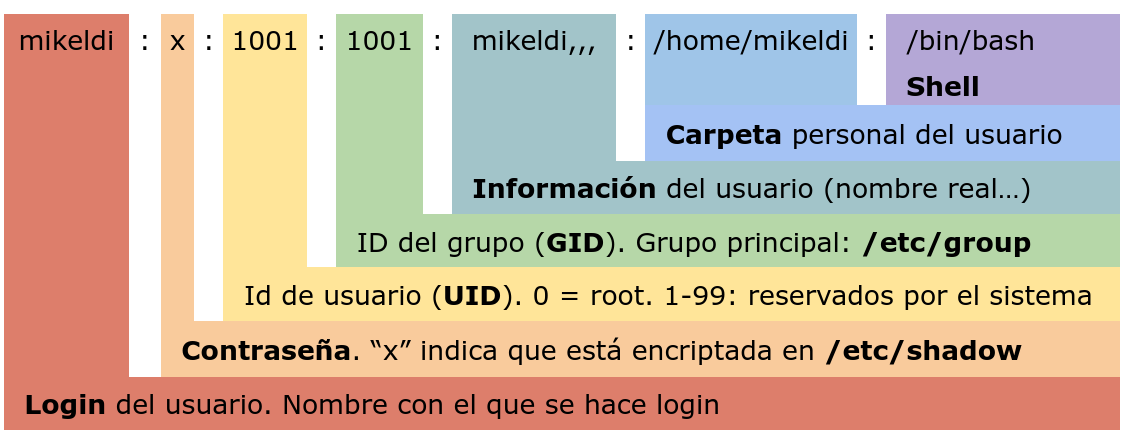
\includegraphics[width=0.7\linewidth]{usuario_tabla.png}
\end{center}


En las primeras versiones GNU/Linux la contraseña de los usuarios aparecía en el propio fichero /etc/passwd, lo que suponía un problema en la seguridad, ya que no estaban cifradas. Actualmente, las contraseñas de los usuarios se almacenan cifradas en el fichero \configfile{ /etc/shadow }. El fichero es similar al passwd, estando separados los apartados por “:”


\begin{center}
  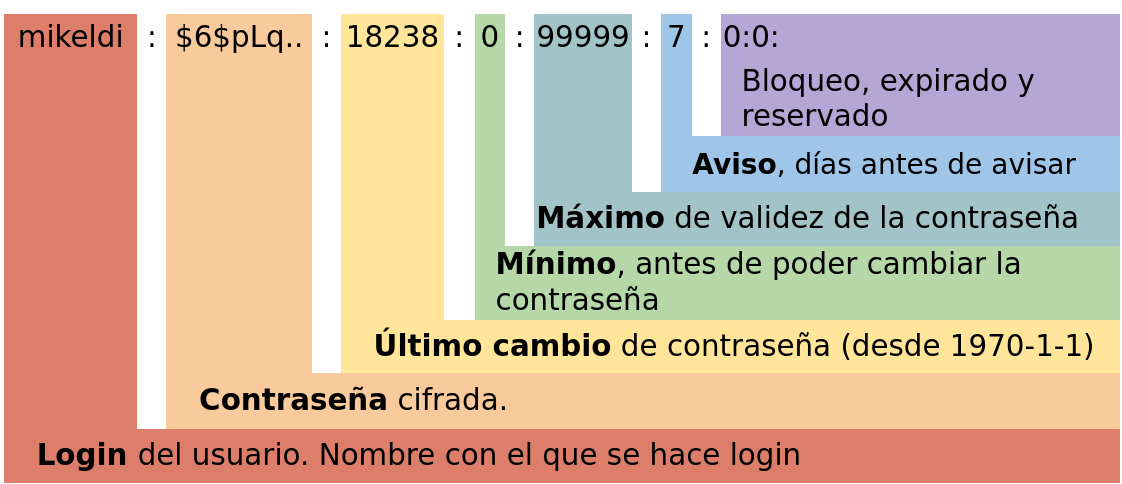
\includegraphics[width=0.7\linewidth]{shadow_tabla.png}
\end{center}


En el apartado de la contraseña podemos saber cierta información acerca de la misma ya que tiene el siguiente formato: \textbf{“\$id\$salt\$hashed”}
\begin{itemize}
    \item \textbf{id}: el algoritmo utilizado para cifrar la contraseña
    \begin{itemize}
        \item \$1\$ – MD5
        \item \$2a\$ – Blowfish
        \item \$2y\$ – Eksblowfish
        \item \$5\$ – SHA-256
        \item \$6\$ – SHA-512
    \end{itemize}
\end{itemize}

Aparte, también podemos encontrarnos con:
\begin{itemize}
    \item \textbf{Contraseña vacía}:  Si no hay contraseña, al pedirnos la contraseña a la hora de hacer login será suficiente con pulsar “intro”.
    \item \textbf{!}, \textbf{*}: la cuenta está bloqueada para la contraseña. El usuario no podrá loguearse utilizando la contraseña. Resulta útil si queremos bloquear el acceso con contraseña pero no con otros métodos (clave pública SSH).
    \item \textbf{*LK*}: cuenta bloqueda. El usuario no podrá loguearse.
    \item \textbf{*NP*}, \textbf{!!}: Nunca se ha puesto una contraseña
\end{itemize}


\section{Gestión de grupos}
En algunas distribuciones GNU/Linux, al crear un usuario directamente nos crea un grupo para el nuevo usuario. En otras, el usuario pertenece al grupo “users”.

Para saber los grupos a los que pertenece un usuario podemos ejecutar el comando \commandbox{ groups }. Los grupos del sistema aparecen en el fichero \configfile{ /etc/group }, y al igual que los ficheros vistos previamente, están separados por “\textbf{:}”.

\begin{center}
  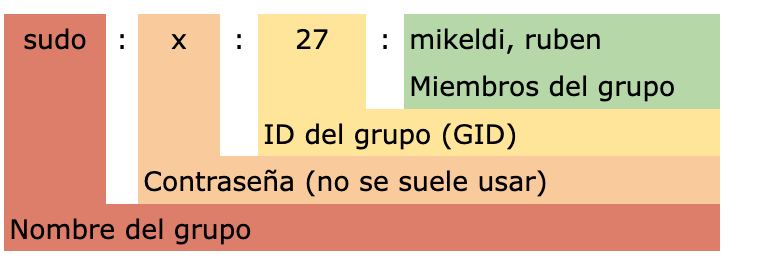
\includegraphics[width=0.6\linewidth]{grupo_tabla.png}
\end{center}

\section{Permisos de ficheros}
En GNU/Linux los ficheros cuentan con 3 tipos de permisos:
\begin{itemize}
    \item lectura (\textbf{r}ead): el usuario puede leer el fichero
    \item escritura (\textbf{w}rite): el usuario puede escribir en el fichero
    \item ejecución (e\textbf{x}ecute): el usuario puede el fichero o puede ver el contenido de un directorio
\end{itemize}


Todos ello para los distintos usuarios que pueden existir en el sistema:
\begin{itemize}
    \item \textbf{dueño del fichero}: la persona que ha creado el fichero
    \item \textbf{grupo}: los usuarios pertenecientes al grupo al que pertenece el fichero tendrán ciertos privilegios
    \item \textbf{el resto de usuarios}: los permisos que tendrán el resto de usuarios que no son ni el dueño ni pertenecen al grupo
\end{itemize}

Todo ello se puede visualizar en el sistema de ficheros si listamos los permisos del fichero:

\begin{mycode}{Ver los permisos de un fichero}{console}{}
ruben@vega:~$ ls -lh fichero.txt
-rw-r--r-- 1 ruben ruben 0 dic  8 19:17 fichero.txt
\end{mycode}

Los permisos se pueden ver en los primeros 10 caracteres:

\begin{center}
  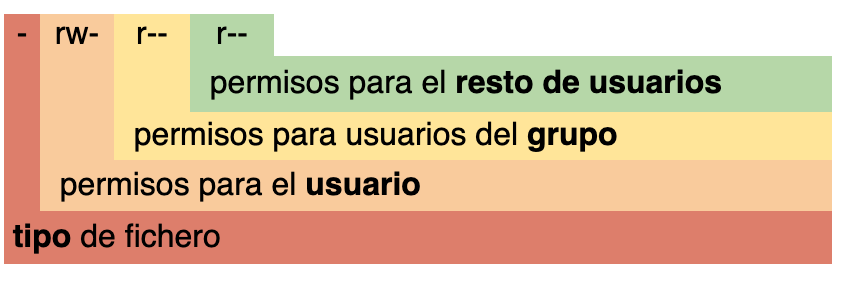
\includegraphics[width=0.7\linewidth]{permisos_fichero.png}
\end{center}

Existen los distintos tipos de ficheros:
\begin{itemize}
    \item \textbf{-} : fichero normal
    \item \textbf{d} : directorio
    \item \textbf{b} : dispositivo de bloque (ejemplo: /dev/sda*)
    \item \textbf{c} : dispositivo de carácter (las consolas. ejemplo: /dev/tty*)
    \item \textbf{s} : socket local
    \item \textbf{p} : tubería (pipe)
    \item \textbf{l} : enlace simbólico (link)
\end{itemize}

\subsection{Permisos especiales}

Existen otros permisos especiales:
\begin{itemize}
    \item \textbf{SUID}: permiso especial que permite que el fichero sea ejecutado con los permisos del dueño del fichero (aunque lo ejecute otro usuario). Se visualiza con una “S” en el permiso de ejecución del dueño  \texttt{-rwSrw-r- -} .
%% TODO: modificar los fondos de los permisos
    \item \textbf{SGID}: permiso especial que permite que el fichero sea ejecutado como el grupo. Aparece una “S” en el permiso de ejecución del grupo: \texttt{-rwx- -S- - -}.

    \item \textbf{STICKY}: si el bit sticky está activado en un directorio sólo el usuario root, el dueño del directorio o el dueño del fichero puede borrar ficheros de dicho directorio. Aparece una “t” en el permiso de ejecución del resto de usuarios: \inlineconsole{d-rwx-rx-r-t}.

\end{itemize}

\subsection{Cambiando permisos y dueños a los ficheros y a los directorios}

Para cambiar los permisos a los ficheros y a los directorios se hace con el comando \textbf{chmod}.

Para cambiar permisos de dueño a los ficheros y a los directorios se hace con el comando \textbf{chown}.

\section{La importancia de “sudo”}
En muchas distribuciones GNU/Linux el usuario no-privilegiado que se crea tiene permiso de “sudo” para poder ejecutar comandos como si se tratara del \textbf{root} (u otro usuario) para poder realizar tareas de administración. Es habitual que en estas distribuciones \textbf{el usuario root no suela tener contraseña}.

Cuando un usuario necesite realizar una tarea como administrador, deberá usar “sudo” antes del comando:

\begin{mycode}{Editar un fichero con permisos de root}{console}{}
ruben@vega:~$ sudo nano /etc/passwd
\end{mycode}

Tras realizar este comando, el sistema nos pedirá la contraseña del usuario con el que lo estemos ejecutando y comprobará que el usuario tiene permisos de “sudo” para poder ejecutar el comando (en este caso: nano).

El comando “\textbf{sudo}” viene de “\textbf{su}per user \textbf{do}” (que en inglés sería: “super usuario haz”), y aunque su uso habitual es el de permitir realizar cualquier comando de administración, la configuración permite mucho más, pudiendo permitir a ciertos usuarios sólo realizar ciertas tareas. Por ejemplo:

\begin{itemize}
    \item Usuario \textbf{ruben}: tendría permisos para poder realizar cualquier comando del sistema.
    \item Usuario \textbf{dba}: sólo tendría permisos para poder realizar el reinicio del sistema de base de datos.
    \item Usuario \textbf{adminweb}: sólo tendría permisos para poder realizar el reinicio del servidor web.
    \item ....
\end{itemize}

De esta manera, la gestión de nuestro servidor estaría basada en múltiples usuarios y cada usuario sólo sería capaz de realizar pequeñas tareas, por lo que la seguridad del servidor sería mayor y limitaría lo que los usuarios puedan realizar.

\subsection{Configurando “sudoers”}
Los permisos de sudo se realizan en el fichero  \configfile{/etc/sudoers} , y para su edición se hace uso del comando \textbf{visudo}, el cual abre el fichero y se asegura que a la hora de guardar la sintaxis es correcta.

Si realizamos cualquier modificación sobre el fichero, éste será tenido en cuenta la próxima vez que se realice la ejecución del comando “sudo”, por lo tanto, no hay que realizar ningún reinicio de servicio.

El fichero \configfile{/etc/sudoers}  tiene permisos de sólo lectura para el usuario root y el grupo root:

\begin{mycode}{Permisos del fichero \faFile \hspace{1pt} /etc/sudoers}{console}{}
root@vega:# ls -lh /etc/sudoers
-r--r----- 1 root root 669 jun  5  2017 /etc/sudoers
\end{mycode}

Un fichero sudoers suele tener el siguiente aspecto:

\begin{mycode}{Contenido del fichero \faFile \hspace{1pt} /etc/sudoers}{bash}{\footnotesize}
Defaults    env_reset
Defaults    mail_badpass
Defaults    secure_path="/usr/local/sbin:/usr/local/bin:/usr/sbin:/usr/bin:/sbin:/bin"

# User privilege specification
root    ALL=(ALL:ALL) ALL

# Allow members of group sudo to execute any command
%sudo   ALL=(ALL:ALL) ALL

# See sudoers(5) for more information on "#include" directives:

#includedir /etc/sudoers.d
\end{mycode}

La línea que más importa en este fichero es la que indica “\textbf{\%sudo   ALL=(ALL:ALL) ALL}” y es explicada en su comentario anterior. Lo que quiere decir es que cualquier usuario que pertenezca al grupo “sudo” podrá realizar cualquier comando del sistema como superusuario. La sintaxis de la línea es:

\begin{itemize}
    \item \textbf{\%sudo}:  cualquier usuario que pertenezca al grupo “sudo”
    \item \textbf{ALL}= : desde cualquier host o IP
    \item \textbf{(ALL:ALL)}: el usuario que ejecuta puede ejecutar el comando como cualquier usuario y cualquier grupo
    \item \textbf{ALL}: puede ejecutar cualquier comando
\end{itemize}

Un ejemplo limitando el uso de sudo a un único comando a un usuario:

\begin{mycode}{Añadimos configuración al fichero \faFile \hspace{1pt} /etc/sudoers}{bash}{}
ruben    ALL=(ALL:ALL) NOPASSWD:/bin/systemctl suspend
\end{mycode}

Con esta línea lo que estamos permitiendo es que el usuario “ruben” puede ejecutar el comando “/bin/systemctl suspend” (suspender el equipo) y sin necesidad de meter contraseña al hacer sudo, gracias a la opción “NOPASSWD”).

\section{Diferencias entre “sudo”, “su” y “su -”}
Como ya se ha comentado en el apartado anterior, “sudo” permite la ejecución de comandos como cualquier usuario, siendo lo habitual ejecutarlo como root. Ahora bien, en entornos donde el usuario root tiene contraseña, nos puede interesar convertirnos en él para realizar tareas sin tener que estar ejecutando “sudo” a cada comando. Al ser root, tendremos que tener especial cuidado.

\subsection{Variables de entorno}
En cualquier sistema operativo existen las denominadas “variables de entorno”. Son variables que cada usuario tiene y sirven para indicar ciertos parámetros que se están utilizando (la SHELL que se está usando), o parámetros que se van a usar a la hora de ejecutar comandos o realizar tareas, ya que se consultan a ellas. En GNU/Linux las variables de entorno se pueden consultar ejecutando:

\begin{mycode}{Vemos las variables de entorno del usuario ruben}{console}{}
ruben@vega:~$ printenv
LANG=es_ES.utf8
LOGNAME=ruben
XDG_VTNR=2
COLORTERM=truecolor
PWD=/home/ruben
DESKTOP_SESSION=gnome
USERNAME=ruben
SHELL=/usr/bin/zsh
PATH=/usr/local/bin:/usr/bin:/bin:/usr/local/games:/usr/games
...
\end{mycode}

Una variable de entorno puede consultarse haciendo:

\begin{mycode}{Consultamos el contenido de la variable \$PATH}{bash}{}
ruben@vega:~$ echo $PATH
/usr/local/bin:/usr/bin:/bin:/usr/local/games:/usr/games

\end{mycode}

Como se puede ver, es con un “\textbf{\$}” y el nombre de la variable en mayúsculas. Existen muchas variables de entorno, y podríamos crear las nuestras propias si así lo necesitáramos.

\subsection{La importancia de “su -”}
Con el comando “\textbf{su}” nos podemos convertir en cualquier otro usuario del sistema siempre y cuando \textbf{conozcamos su contraseña}. Hay que notar la diferencia respecto a “\textbf{sudo}” que cuando lo ejecutamos nos pide \textbf{nuestra contraseña}.

\textbf{Al ejecutar “su” nos convertimos en el usuario root} (o ejecutando “su usuario2”, nos convertimos en el usuario2), \textbf{pero no hacemos uso de sus variables de entorno}, si no que seguimos  con las variables de entorno del usuario que éramos previamente.
Para convertirnos en el usuario y que obtengamos sus variables de entorno es necesario ejecutar “\textbf{su -}”, o lo que es lo mismo: “\textbf{su -l}”, que el manual nos dice: “\textit{Start the shell as a login shell with an environment similar to a real login}”. Por ejemplo:

\begin{mycode}{Consultamos el contenido de la variable \$PATH en distintas situaciones}{bash}{}
ruben@vega:~$ echo $PATH
/usr/local/bin:/usr/bin:/bin:/usr/local/games:/usr/games

ruben@vega:~$ su
Contraseña:

root@vega:/home/ruben# echo $PATH
/usr/local/bin:/usr/bin:/bin:/usr/local/games:/usr/games

root@vega:/home/ruben# exit

ruben@vega:~$ su -
Contraseña:

root@vega:~# echo $PATH
/usr/local/sbin:/usr/local/bin:/usr/sbin:/usr/bin:/sbin:/bin

\end{mycode}

El usuario “ruben” tiene unos valores en la variable de entorno PATH (es la variable que se encarga de tener las rutas de los ejecutables de los programas). Al convertirse en root haciendo uso de “su”, y mirar la variable PATH, podemos observar que es igual que el usuario prueba.

Ahora bien, si a la hora de convertirse en root hace uso de “su -”, se puede ver cómo la variable PATH obtiene otros valores, siendo lo más significativo que aparecen las rutas “/usr/local/sbin” y “/usr/sbin” que son las rutas donde se almacenan los ejecutables que (en principio) sólo deberían ejecutarse como administrador del sistema.



    \chapter{Comandos de administración básica en GNU/Linux}
En este documento vamos a recopilar comandos que nos pueden ser útiles a la hora de usar un sistema GNU/Linux y realizar su administración.

\section{Comandos sobre el sistema de ficheros}
A continuación unos comandos básicos para utilizar sobre el sistema de ficheros.

\begin{mycode}{Listar el contenido del directorio donde nos encontramos}{console}{}
ruben@vega:~$ ls
Descargas   Escritorio  Música      Público
Documentos  Imágenes    Plantillas  Vídeos
\end{mycode}

\begin{mycode}{Listar el directorio actual, versión “long”}{console}{}
ruben@vega:~$ ls -l
total 36K
drwxr-xr-x 2 ruben ruben 4,0K nov 12  2022 Descargas
drwxr-xr-x 2 ruben ruben 4,0K dic  6 09:50 directorio1
drwxr-xr-x 2 ruben ruben 4,0K nov 12  2022 Documentos
drwxr-xr-x 2 ruben ruben 4,0K nov 12  2022 Escritorio
drwxr-xr-x 2 ruben ruben 4,0K nov 12  2022 Imágenes
drwxr-xr-x 2 ruben ruben 4,0K nov 12  2022 Música
drwxr-xr-x 2 ruben ruben 4,0K nov 12  2022 Plantillas
drwxr-xr-x 2 ruben ruben 4,0K nov 12  2022 Público
drwxr-xr-x 2 ruben ruben 4,0K nov 12  2022 Vídeos
\end{mycode}


\begin{mycode}{Crear un nuevo directorio}{console}{}
ruben@vega:~$ mkdir directorio1
ruben@vega:~$ ls
Descargas    Documentos  Imágenes  Plantillas  Vídeos
directorio1  Escritorio  Música    Público
\end{mycode}

\begin{mycode}{Borrar un directorio que está vacío}{console}{}
ruben@vega:~$ rmdir directorio1
\end{mycode}


\begin{mycode}{Editar un fichero}{console}{}
ruben@vega:~$ nano fichero.txt
\end{mycode}

\begin{mycode}{Obtener el contenido de un fichero de texto}{console}{}
ruben@vega:~$ cat fichero.txt
hola, qué tal
\end{mycode}

\begin{mycode}{Paginar el contenido de un fichero de texto}{console}{}
ruben@vega:~$ more fichero.txt
hola, qué tal
...
\end{mycode}

\begin{mycode}{Borrar un fichero}{console}{}
ruben@vega:~$ rm fichero.txt
\end{mycode}

\begin{mycode}{Borrar un directorio y todo el contenido que tiene dentro. ¿Diferencias?}{console}{}
ruben@vega:~$ rm -r directorio2
ruben@vega:~$ rm -fr directorio2
\end{mycode}

\begin{mycode}{Buscar por un contenido dentro de un fichero}{console}{}
ruben@vega:~$ grep hola fichero.txt
\end{mycode}


\section{Comandos de red}
Para ver los interfaces de red y las direcciones IP que tienen

\begin{mycode}{Obtener los interfaces y las IPs}{console}{}
ruben@vega:~$ ip a
1: lo: <LOOPBACK,UP,LOWER_UP> mtu 65536
link/loopback 00:00:00:00:00:00 brd 00:00:00:00:00:00
inet 127.0.0.1/8 scope host lo

2: enp4s0: <BROADCAST,MULTICAST,UP,LOWER_UP> mtu 1500
link/ether 1a:8a:1c:ff:25:15 brd ff:ff:ff:ff:ff:ff
inet 192.168.1.99/24 brd 192.168.1.255 scope global enp4s0
\end{mycode}

Para ver la ruta por defecto (el gateway o puerta de enlace).

\begin{mycode}{Obtener la puerta de enlace}{console}{}
ruben@vega:~$ ip route show default
default via 192.168.1.1 dev enp4s0 onlink
\end{mycode}

Ver los puertos TCP y servicios que están a la escucha en nuestro servidor
\begin{mycode}{Listar los puertos TCP a la escucha}{console}{}
root@vega:~# ss -pntal
\end{mycode}

\section{Comandos sobre procesos}
Listar todos los procesos
\begin{mycode}{Listar todos los procesos}{console}{}
root@vega:~# ps aux
\end{mycode}

Listar todos los procesos en forma de árbol (para saber de quién son hijos)
\begin{mycode}{Listar todos los procesos en forma de árbol}{console}{}
root@vega:~# pstree -p
\end{mycode}

Matar un proceso (donde PID es el identificador del proceso).
\begin{mycode}{Matar un proceso}{console}{}
root@vega:~# kill -9 PID
\end{mycode}

\section{Estado de la carga y memoria del servidor}
Para ver los procesos y su estado por consumo de CPU, RAM…
\begin{mycode}{Ver el estado del servidor}{console}{}
root@vega:~# top
\end{mycode}

Para ver los procesos y su estado por consumo de CPU, RAM… es necesario instalar este paquete
\begin{mycode}{Ver el estado del servidor}{console}{}
root@vega:~# htop
\end{mycode}

\section{Comandos sobre servicios (systemd/systemctl)}
GNU/Linux cuenta con un sistema unificado (\textbf{systemd}) para administrar el sistema y los servicios que tenemos en nuestro servidor. Dado que es una pieza fundamental en el sistema operativo, debemos de conocer ciertos comandos para poder desempeñar tareas con él.

Listar todos los servicios/unidades
\begin{mycode}{Listar todos los servicios}{console}{}
root@vega:~# systemctl
\end{mycode}

Comprobar si algún servicio ha fallado
\begin{mycode}{Comprobar servicios que han fallado}{console}{}
root@vega:~# systemctl --failed
\end{mycode}

Comprobar el estado de un servicio concreto (en este caso, ssh)
\begin{mycode}{Comprobar servicios que han fallado}{console}{}
root@vega:~# systemctl status ssh
\end{mycode}

Parar un servicio concreto
\begin{mycode}{Parar un servicio concreto}{console}{}
root@vega:~# systemctl stop ssh
\end{mycode}

Arrancar un servicio concreto
\begin{mycode}{Arrancar un servicio concreto}{console}{}
root@vega:~# systemctl start ssh
\end{mycode}

Ver los logs de todo el sistema
\begin{mycode}{Ver los logs del sistema}{console}{}
root@vega:~# journalctl
\end{mycode}

Ver los logs de un servicio concreto (en este caso, ssh)
\begin{mycode}{Ver los logs del sistema}{console}{}
root@vega:~# journalctl -u ssh
\end{mycode}

Ver los logs del kernel
\begin{mycode}{Ver los logs del kernel}{console}{}
root@vega:~# journalctl -k
\end{mycode}


\section{Comandos para instalar/desinstalar paquetes}

Los comandos que se van a exponer aquí sirven para las distribuciones que utilizan el sistema de paquetes \href{https://es.wikipedia.org/wiki/Advanced_Packaging_Tool}{APT (Advanced Packaging Tool)} que está presente en las distribuciones derivadas de \href{https://www.debian.org/}{Debian}, como por ejemplo Ubuntu.


\begin{mycode}{Sincroniza el índice de paquetes local con lo que está en los repositorios remotos configurados en \textbf{/etc/apt/sources.list}}{console}{}
root@vega:~# apt update
\end{mycode}

\begin{mycode}{Instala las versiones más nuevas de los paquetes que ya tenemos instalados}{console}{}
root@vega:~# apt upgrade
\end{mycode}


\begin{mycode}{Instala las versiones más nuevas de los paquetes  teniendo en cuenta las dependencias de los mismos y solucionando posibles conflictos.}{console}{}
root@vega:~# apt full-upgrade
\end{mycode}


\section{Comandos para apagar/reiniciar}

Para realizar el apagado o reinicio de un equipo se pueden utilizar varios comandos distintos.

\begin{mycode}{Reiniciar el equipo}{console}{}
root@vega:~# reboot
\end{mycode}

\begin{mycode}{Apagar el equipo en un minuto}{console}{}
root@vega:~# shutdown
\end{mycode}

\begin{mycode}{Apagar el equipo ahora}{console}{}
root@vega:~# shutdown now
\end{mycode}

\begin{mycode}{Suspender el equipo}{console}{}
root@vega:~# systemctl suspend
\end{mycode}

    \part{Anexos}

    \graphicspath{{../../../anexos/virtualbox_networking/img}}
    \chapter{Virtualbox y adaptadores de red}

\section{Introducción}
\href{https://www.virtualbox.org/}{Virtualbox} es una herramienta de virtualización para crear máquinas virtuales de manera sencilla. Es multiplataforma por lo que se puede utilizar en Windows, MacOS y Linux y aparte, es \hyperlink{software_libre}{Software Libre}.

Este documento no va a entrar en detalle en cómo se crean las máquinas virtuales, sino que va a explicar los distintos modos y adaptadores de red que puede tener una máquina virtual en este sistema de virtualización.

\section{Adaptadores de red}
Virtualbox permite que cada máquina virtual cuente con hasta cuatro adaptadores de red, lo que comúnmente se llaman interfaces o NIC (network interface controller).

Al crear las máquinas virtuales sólo tienen un único adaptador activo y suele estar configurado en modo NAT, pero tal como se ve a continuación, en el desplegable se puede ver que existen otras opciones:

\begin{center}
    \vspace{-10pt}
    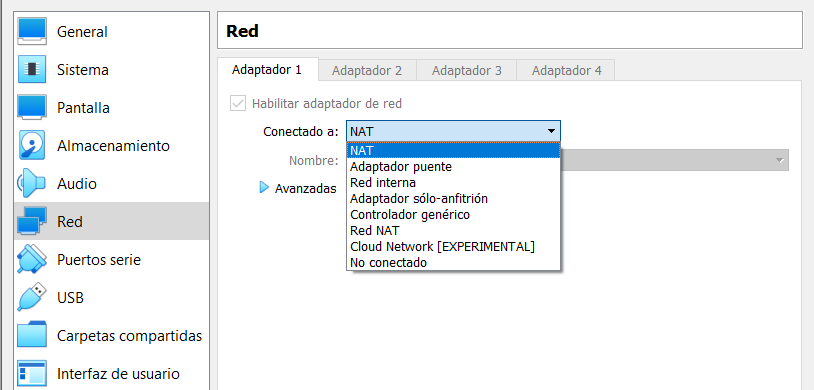
\includegraphics[frame,width=0.7\linewidth]{virtualbox_1.png}
    \vspace{-20pt}
\end{center}

En la \href{https://www.virtualbox.org/manual/ch06.html}{documentación oficial} aparece la explicación de los distintos modos, y es buena práctica leer y entender la documentación del software que utilizamos. También hay que entender que cada tipo de adaptador contará con una serie de ventajas y una serie de limitaciones que aparecen reflejadas en la documentación. Estos modos son comunes a otros  sistemas de virtualización (VmWare, Proxmox, …), pero el nombre o el modo de uso puede variar así como las posibles limitaciones que puedan existir.

A continuación se va a dar una pequeña introducción a cada tipo de adaptador.

\subsection{Adaptador puente}
Es el tipo de adaptador que se usará si queremos que las máquinas virtuales aparezcan en la red física como si fueran un equipo más. Para poder entenderlo de mejor manera, podríamos pensar que este tipo de adaptador lo que hace es crear un “switch virtual” entre las máquinas virtuales y el interfaz físico, por lo que es como si fueran un equipo más en la red física.

Si el equipo físico anfitrión cuenta con más de un NIC (por ejemplo, en un portátil el NIC por cable y el NIC wifi) tendremos que elegir en la máquina virtual sobre qué NIC queremos hacer el puente. En la siguiente imagen en el desplegable sólo se puede seleccionar un interfaz porque el equipo sólo cuenta con un NIC físico.

\begin{center}
    \vspace{-10pt}
    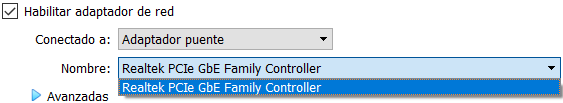
\includegraphics[frame,width=0.7\linewidth]{virtualbox_2.png}
    \vspace{-20pt}
\end{center}

Es el método utilizado cuando virtualizamos servidores, ya que podrán dar sus servicios a toda la red.

\begin{center}
    \vspace{-10pt}
    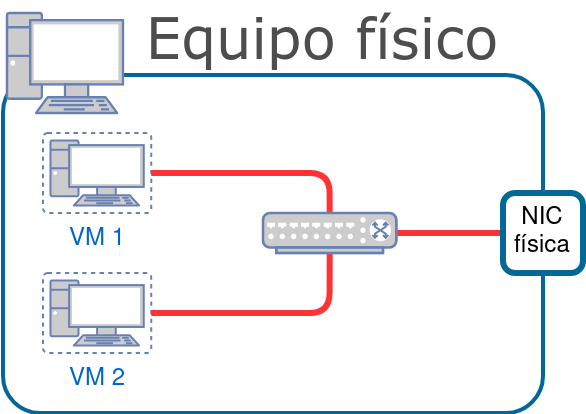
\includegraphics[width=7cm]{virtualbox-bridge.png}
    \vspace{-10pt}\captionof{figure}{Red como Adaptador Puente}
    \vspace{-20pt}
\end{center}

\subsection{NAT}
Cada máquina virtual contará con su propio “router virtual” que hará NAT, y por eso todas las máquinas virtuales que usen este modo suelen tener la misma IP, pero no pertenecen a la misma red.
Por defecto no se puede realizar conexión desde la red física al equipo virtualizado.

\begin{center}
    \vspace{-10pt}
    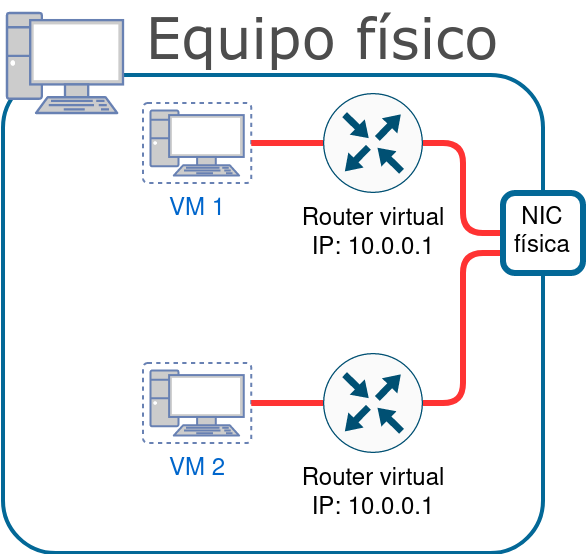
\includegraphics[width=7cm]{virtualbox-NAT.png}
    \vspace{-10pt}\captionof{figure}{Red en modo NAT}
    \vspace{-20pt}
\end{center}

\subsection{Red interna}
Este tipo de adaptador lo que hace es “crear” un “switch virtual” que unirá las distintas máquinas virtuales que estén conectadas al nombre de esa red interna.

En el siguiente ejemplo la VM1 tiene 2 NICs, cada una con una red interna distinta. La VM2 tiene un NIC conectado a una de las redes internas creadas previamente y VM3 está conectada a la otra red interna.

Virtualbox no se encarga de dar IPs en estas redes, por lo que deberemos configurar cada interfaz de la máquina virtual con el direccionamiento que nos interese.

Este método se utiliza si queremos comunicar máquinas virtuales entre sí y que estén aisladas, ya que no podrán conectarse con el exterior, ni siquiera con el propio equipo físico.

\begin{center}
    \vspace{-10pt}
    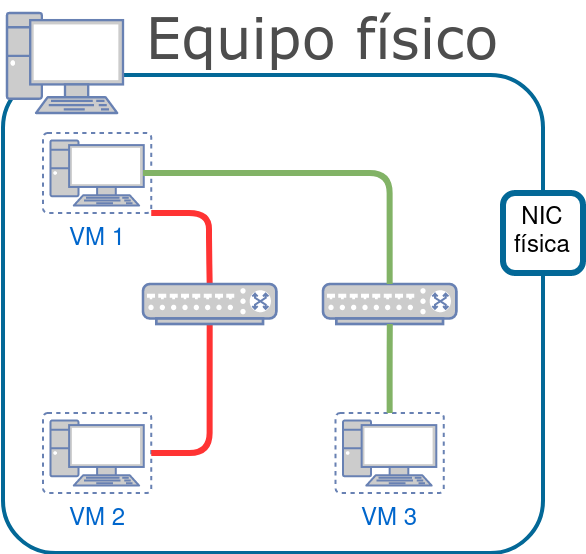
\includegraphics[width=7cm]{virtualbox-red_interna.png}
    \vspace{-10pt}\captionof{figure}{Red Interna}
    \vspace{-20pt}
\end{center}

\subsection{Red NAT}
Podría definirse como una mezcla de NAT y red interna. Las máquinas virtuales podrán pertenecer a una única red, se podrán comunicar entre ellas, estarán detrás de un NAT de la red física y se podrán comunicar con el exterior.

Para poder usar ese modo hay que crear la “red NAT” en Virtualbox yendo a “\textit{Archivo → Preferencias → Red}” y ahí se creará las redes NAT que queramos con el direccionamiento interno que nos interese.

\begin{center}
    \vspace{-10pt}
    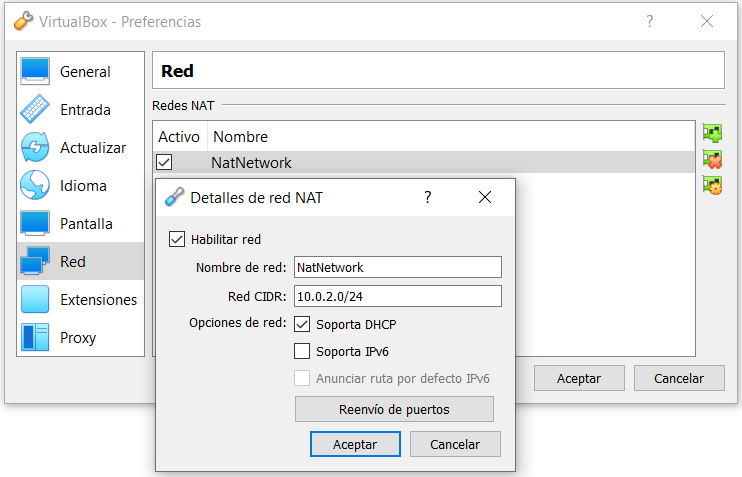
\includegraphics[width=8cm]{virtualbox-red-NAT_config.png}
    \vspace{-20pt}
\end{center}

A la hora de crear la máquina virtual y elegir la opción “Red NAT” se podrá elegir entre las redes creadas en el paso anterior.

\begin{center}
    \vspace{-10pt}
    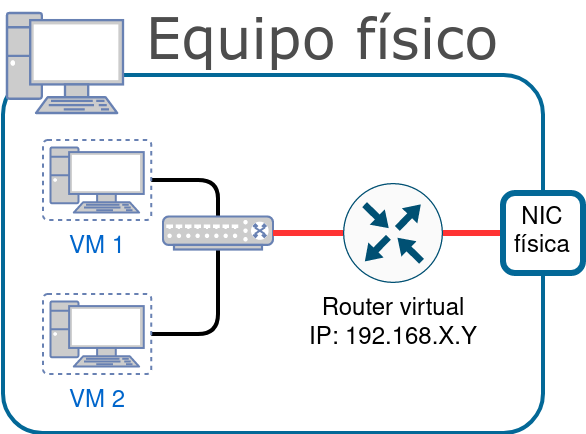
\includegraphics[width=7cm]{virtualbox-red-NAT.png}
    \vspace{-10pt}\captionof{figure}{Red NAT}
    \vspace{-20pt}
\end{center}

\subsection{Adaptador sólo-anfitrión}
Este tipo de adaptador es similar al de “red interna” pero con la posibilidad de comunicarse con el equipo físico anfitrión. En el equipo físico se crea un interfaz virtual y a través de él se podrá comunicar con las máquinas virtuales.

\begin{center}
    \vspace{-10pt}
    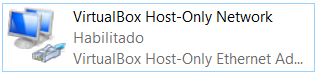
\includegraphics[width=7cm]{virtualbox-host_only_nic.png}
    \vspace{-20pt}
\end{center}

El direccionamiento que existe entre las VMs y el host se define en Virtualbox, dentro de “\textit{Archivo → \textbf{Administrador de red de anfitrión}}”. Las máquinas virtuales podrán coger IP de ese direccionamiento  por DHCP.

Mismo uso que “red interna” pero añadiendo la opción de comunicarnos con el host anfitrión.

\begin{center}
    \vspace{-10pt}
    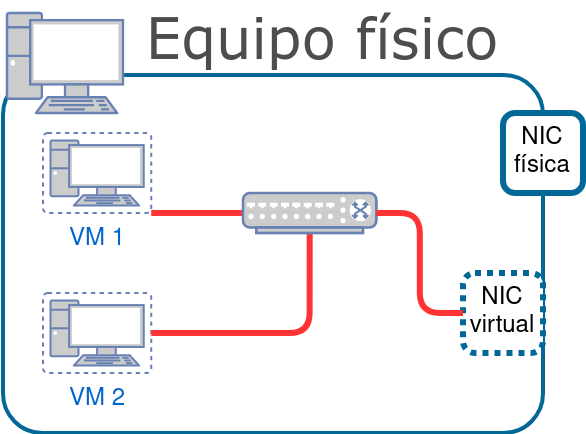
\includegraphics[width=7cm]{virtualbox-host_only.png}
    \vspace{-10pt}\captionof{figure}{Red en modo “Sólo Anfitrión”}
    \vspace{-20pt}
\end{center}

\section{Resumen de los adaptadores}
A continuación se expone una tabla que resume los distintos tipos de adaptadores que existen y la conectividad posible entre las máquinas virtuales que usan esos adaptadores y el host anfitrión (\href{https://www.virtualbox.org/manual/ch06.html#networkingmodes}{fuente}).

\begin{center}
    \vspace{-10pt}
    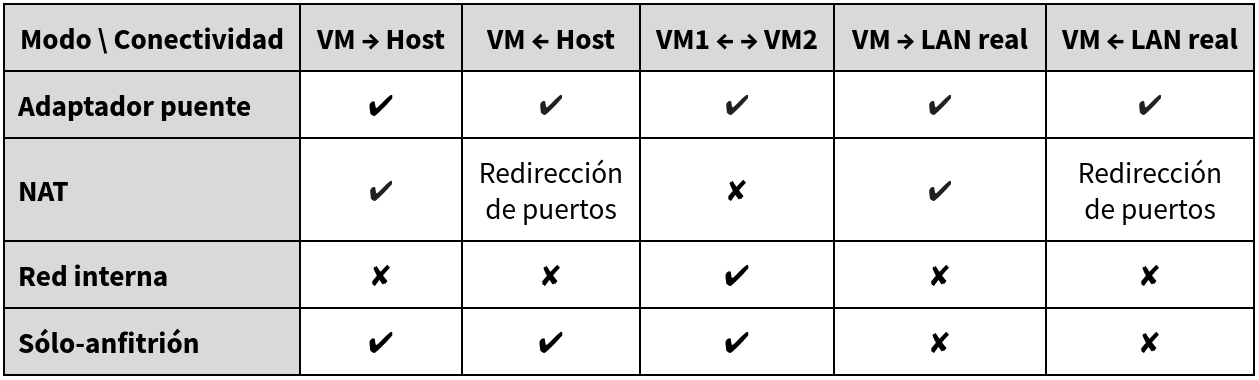
\includegraphics[width=\linewidth]{virtualbox_tabla.png}
    \vspace{-20pt}
\end{center}

En la \href{https://www.virtualbox.org/manual/ch06.html#natforward}{documentación} se explica cómo realizar la redirección de puertos.


\clearpage

    \hypertarget{tabla_conversiones_directas}{}

\chapter{Sistemas de numeración: tabla de conversión}
La siguiente tabla sirve a modo de resumen de los sistemas de numeración.

\infobox{\textbf{Esta tabla no hay que aprenderla de memoria}.
    Hay que entender los sistemas de numeración y de esta manera se puede crear. }

\begin{yukitblr}{X X X X}
    Decimal       &      Binario     &      Octal    & Hexadecimal \\

    $  0_{(10} $  & $      0_{(2} $  & $  0_{(8} $   & $  0_{(16} $  \\
    $  1_{(10} $  & $      1_{(2} $  & $  1_{(8} $   & $  1_{(16} $  \\
    $  2_{(10} $  & $     10_{(2} $  & $  2_{(8} $   & $  2_{(16} $  \\
    $  3_{(10} $  & $     11_{(2} $  & $  3_{(8} $   & $  3_{(16} $  \\
    $  4_{(10} $  & $    100_{(2} $  & $  4_{(8} $   & $  4_{(16} $  \\
    $  5_{(10} $  & $    101_{(2} $  & $  5_{(8} $   & $  5_{(16} $  \\
    $  6_{(10} $  & $    110_{(2} $  & $  6_{(8} $   & $  6_{(16} $  \\
    $  7_{(10} $  & $    111_{(2} $  & $  7_{(8} $   & $  7_{(16} $  \\
    $  8_{(10} $  & $   1000_{(2} $  & $ 10_{(8} $   & $  8_{(16} $  \\
    $  9_{(10} $  & $   1001_{(2} $  & $ 11_{(8} $   & $  9_{(16} $  \\
    $ 10_{(10} $  & $   1010_{(2} $  & $ 12_{(8} $   & $  A_{(16} $  \\
    $ 11_{(10} $  & $   1011_{(2} $  & $ 13_{(8} $   & $  B_{(16} $  \\
    $ 12_{(10} $  & $   1100_{(2} $  & $ 14_{(8} $   & $  C_{(16} $  \\
    $ 13_{(10} $  & $   1101_{(2} $  & $ 15_{(8} $   & $  D_{(16} $  \\
    $ 14_{(10} $  & $   1110_{(2} $  & $ 16_{(8} $   & $  E_{(16} $  \\
    $ 15_{(10} $  & $   1111_{(2} $  & $ 17_{(8} $   & $  F_{(16} $  \\
    $ 16_{(10} $  & $  10000_{(2} $  & $ 20_{(8} $   & $ 10_{(16} $  \\
    $ 17_{(10} $  & $  10001_{(2} $  & $ 21_{(8} $   & $ 11_{(16} $  \\
    ... & ... & ... & ... \\
    $ 29_{(10} $  & $  11101_{(2} $  & $ 35_{(8} $   & $ 1D_{(16} $  \\
    $ 30_{(10} $  & $  11110_{(2} $  & $ 36_{(8} $   & $ 1E_{(16} $  \\
    $ 31_{(10} $  & $  11111_{(2} $  & $ 37_{(8} $   & $ 1F_{(16} $  \\
    $ 32_{(10} $  & $ 100000_{(2} $  & $ 40_{(8} $   & $ 20_{(16} $  \\
\end{yukitblr}

\clearpage

    \graphicspath{{../../../anexos/}}
    \chapter{Glosario}

A continuación se expone un glosario de términos con sus correspondientes definiciones:

\begin{description}
    \hypertarget{altadisponibilidad}{}
    \item[Alta Disponibilidad:] Es un diseño de arquitectura de sistemas y la implementación que asegura que el servicio instalado y otorgado sea funcional sin que haya parada en el mismo. Esta arquitectura trata de que no haya ningún \hyperlink{spf}{\textit{single point of failure} (punto único de fallo)} en la misma.

    \hypertarget{cluster}{}
    \item[Clúster:] Se denomina clúster a un conjunto de ordenadores unidos entre sí mediante conectividad de red que actúan como si de un único servidor se tratara. Dependiendo del tipo de clúster que se va a crear, debe de ser pensado desde el diseño del servicio, ya que es la aplicación o servicio quién se encarga de crear el clúster (como ocurre con MySQL Cluster).

    \hypertarget{dependencia_software}{}
    \item [Dependencia de software:] Cuando se crea cualquier tipo de software lo habitual es hacer uso de otro software (librerías de seguridad, acceso a disco, codecs de vídeo, librerías 3D…) que son necesarias para el correcto funcionamiento de nuestro programa. Este otro software (que puede ser propio o ajeno) se denomina \textbf{dependencia}, ya que sin él, nuestro programa no funcionará y es necesario que exista en el sistema para hacer funciona nuestro programa.

    En las \hyperlink{distribucion_gnu_linux}{distribuciones GNU/Linux} se hace uso de los denominados \hyperlink{paquete_de_software}{paquetes de software} en los cuales se indican las dependencias que necesitan para funcionar y que por tanto se instalarán a la par que el programa elegido, por lo que nos aseguramos que el software instalado funcionará en cuanto termine la instalación.

    En caso de descargar un software ajeno de los \hyperlink{repositorio_de_software}{repositorios} oficiales de la distribución, es posible que necesitemos completar esas dependencias por nuestra cuenta, pero hoy en día es habitual que los creadores de software lo tengan en cuenta y esas dependencias estén en los repositorios oficiales.

    \hypertarget{distribucion_gnu_linux}{}
    \item [Distribución GNU/Linux:] Es una distribución de software basada en el núcleo Linux que incluye software \hyperlink{gnu}{GNU} para componer un Sistema Operativo que pueda ser utilizado por los usuarios. Cada distribución suele \hyperlink{paquete_de_software}{empaquetar el software} en un formato propio que aparte del propio software indica las \hyperlink{dependencia_de_software}{dependencias} de software que necesita para funcionar, por lo que hace que la instalación del software se realice de manera sencilla. El software de la distribución está almacenado en los \hyperlink{repositorio_de_software}{repositorios de software} oficiales de la distribución.

    Las distribuciones suelen estar orientadas para un uso generalizado, pero es cierto que algunas, por su historia o por su manera de entender el empaquetado de software, se necesitan más conocimientos, pero hoy en día no es lo habitual.

    Existen muchas distribuciones GNU/Linux, pero las que podríamos destacar son \hyperlink{ubuntu}{Ubuntu}, Debian, Red Hat y CentOS, que son las de mayor uso hoy en día a nivel profesional.

    \hypertarget{escalado_horizontal}{}
    \item[Escalado Horizontal:] Se llama escalado horizontal a la infraestructura que crece de manera horizontal añadiendo más servidores del mismo servicio. Estos servidores serán accesibles mediante un proxy o de manera directa, y todos contarán con el mismo servicio (web, base de datos, …). No confundir con un clúster, ya que la relación de los servidores en el escalado horizontal no tienen por qué ir en clúster.

    \hypertarget{escalado_vertical}{}
    \item[Escalado Vertical:] Es el incremento de hardware de un servidor. Supongamos que un servidor empieza a tener problemas de carga, pues con el escalado vertical se le añadiría más RAM, más procesador y/o discos duros más rápidos (en caso de ser una máquina virtual sería sencillo, en caso contrario habría que realizar la migración a un servidor nuevo).

    \hypertarget{gnu}{}
    \item[GNU:] Del acrónimo \textbf{GNU’s Not Unix} (GNU no es Unix) es un sistema operativo y un conjunto de programas libres cuyo origen surgió de la idea de crear un sistema operativo Unix basado en \hyperlink{software_libre}{Software Libre}.

    El desarrollo de GNU nació en 1983 por Richard Stallman comenzando por el compilador GCC, al que se fueron uniendo todo tipo de software y creando la Free Software Foundation (o FSF, fundación por el software libre) la cual creó la \hyperlink{licencias_libres}{licencia libre} más conocida actualmente: la \textbf{GPL} (GNU General Public License).

    El proyecto GNU avanzó en el tiempo y creó el kernel Hurd, pero bien es cierto que nunca llegó a ser funcional del todo y actualmente el kernel más utilizado es Linux, pero no es el único, ya que el software GNU también es usado en conjunto con otros kernels como son los \textbf{*BSD}, de ahí la importancia que cuando hacemos referencia al sistema operativo se haga uso de \hyperlink{gnu_linux}{GNU/Linux}.

    \hypertarget{gnu_linux}{}

    \itemimage{GNU/Linux:}{r}{0.21}
    {img/Gnulinux.svg.png}
    {\href{https://es.wikipedia.org/wiki/GNU/Linux\#/media/Archivo:Gnulinux.svg}{GNU/Linux: Wikipedia}}
    {
        Aunque comúnmente solemos llamar a las \hyperlink{distribucion_gnu_linux}{distribuciones} como “Linux” esto no suele ser correcto ya que en la distribución aparte del kernel va un conjunto enorme de software del proyecto GNU. Por lo tanto, lo ideal siempre es hacer uso del nombre completo GNU/Linux.

        El proyecto \hyperlink{gnu}{GNU} y sus herramientas y software son usados con otros kernels como son los *BSD en distribuciones como FreeBSD u OpenBSD. También existen versiones con kernel BSD para la distribución Debian, por lo que en ese caso sería “Debian GNU/BSD”.
    }


    \hypertarget{json}{}
    \item[JSON:] Es un formato de texto sencillo para el intercambio de datos. Aunque originalmente fue creado como notación de objetos para Javascript, su amplia utilización ha hecho que sea utilizado como alternativa a XML.


    \hypertarget{licencias_libres}{}
    \item[Licencias libres:] Una licencia de software es un contrato entre el creador (o el titular de los derechos de autor) del software y el usuario. Todo software que usamos suele exigir la lectura de esta licencia y es por ello muy importante conocer qué se puede y no se puede hacer con dicho software.

    Las licencias libres son aquellas que nos permiten hacer con el software lo que las cuatro libertades del \hyperlink{software_libre}{Software Libre} exige.

    Entre las licencias libres más utilizadas hoy en día están la GPL (General Public License del proyecto \hyperlink{gnu}{GNU}), la Apache License, algunas de las versiones de las licencias Creative Commons, …


    \hypertarget{linux}{}
    \item[Linux:] Creado originalmente por Linus Torvalds en 1991 y actualmente desarrollado por cientos de desarrolladores de todo el mundo, Linux es el núcleo (o kernel) gratuito y libre similar al núcleo de los sistemas operativos Unix.

    Comenzó como un proyecto personal de Linus (siendo estudiante universitario) para su ordenador 386 y actualmente está portado a \href{https://es.wikipedia.org/wiki/Portabilidad\_del\_n\%C3\%BAcleo\_Linux\_y\_arquitecturas\_soportadas}{decenas de plataformas hardware}. Es el proyecto más grande y ambicioso del \hyperlink{software_libre}{Software Libre}, aunque originalmente no se permitía el uso comercial del mismo (hasta la versión 0.12).

    Al poco tiempo de comenzar su desarrollo el proyecto \hyperlink{gnu}{GNU} lo adoptó como su kernel naciendo lo que actualmente conocemos como \hyperlink{gnu_linux}{GNU/Linux} y con ello cientos de \hyperlink{distribucion_gnu_linux}{distribuciones}.

    Es un núcleo de tipo monolítico que permite la carga de módulos en tiempo de ejecución


    \hypertarget{lts}{}
    \item[LTS:] Del inglés \textit{\textbf{L}ong \textbf{T}erm \textbf{S}upport} (en castellano “soporte a largo plazo”), es una característica en informática que hace referencia a versiones especiales de software que contarán con un soporte más largo del habitual, por lo que serán las versiones idóneas para usar en servidores.

    Estas versiones suelen contar con actualizaciones de seguridad, pero no con cambios notorios en la forma del software para fomentar la fiabilidad del mismo. Lo habitual es utilizar este tipo de versiones en servidores, que aunque puedan no tener las últimas modificaciones de las versiones más recientes del software, nos aseguramos la fiabilidad. Esto hace que tengamos que decidir si es necesario contar con las características de las últimas versiones (ya sea nuevos servicios, opciones nuevas, velocidad, … ) o si preferimos contar con una versión que tendrá un ciclo de vida más longevo pero con actualizaciones de seguridad.

    Es habitual verlo en proyectos de \hyperlink{software_libre}{Software Libre}, como ejemplos podemos tomar el kernel \hyperlink{linux}{Linux} (actualmente la versión 5.4.58 es la denominada LTS) y la distribución \hyperlink{ubuntu}{Ubuntu} (en este caso la versión 20.04).


    \hypertarget{paquete_de_software}{}
    \item[Paquetes de Software:] Un paquete de software no es más que una manera de poder distribuir el software creado. En \hyperlink{distribucion_gnu_linux}{distribuciones GNU/Linux} estos paquetes determinan las \hyperlink{dependencia_software}{dependencias} que necesitan para que su instalación sea lo más sencilla posible.

    Lo habitual es que estos paquetes estén gestionados mediante un sistema de gestión propio para conocer cuáles están instalados, sus dependencias, desinstalarlos de manera sencila...

    No sólo se usa en distribuciones GNU/Linux, ya que varios lenguajes de programación hacen lo propio para distribuir software en forma de paquetes. Como ejemplos:
    \begin{itemize}
        \item En distribuciones GNU/Linux tenemos APT, Yum, Zypper, Portage, ...
        \item En lenguajes de programación tenemos Gem para Ruby, Eggs para Python, CPAN en Perl, ...
    \end{itemize}


    \hypertarget{repositorio_de_software}{}
    \item[Repositorio de Software:] Se podría denominar repositorio como el almacén donde se guardan los \hyperlink{paquete_de_software}{paquetes de software}. Las \hyperlink{distribucion_gnu_linux}{distribuciones GNU/Linux} cuentan con sus repositorios oficiales, donde se almacena el software para cada versión que tiene la distribución.

    Aparte del software que podemos instalar, también cuentan con un índice para saber los paquetes y las versiones que se almacena en ellos. Este índice es necesario que lo actualicemos de manera periódica (en Ubuntu ejecutando: “apt update”) ya que gracias a él sabremos si tenemos que realizar actualizaciones de los paquetes instalados.

    También podemos utilizar repositorios externos al de la distribución, repositorios oficiales de un software por ejemplo, que nos permiten instalar la última versión de ese software sobre nuestra distribución. Cuando un paquete con el mismo nombre existe en distintos repositorios, siempre se instalará del repositorio que tenga la versión más nueva.

    No es buena práctica, y \textbf{está completamente desaconsejado}, mezclar repositorios de distribuciones distintas aunque el gestor de paquetes sea el mismo (usar repositorios de Debian en Ubuntu o viceversa).


    \hypertarget{spf}{}
    \item[Single Point of Failure:] O punto único de fallo, es un componente de un sistema que tras un fallo en su funcionamiento ocasiona un fallo global en el sistema completo, dejándolo inoperante. Un SPOF puede ser un componente de hardware, software o eléctrico.


    \hypertarget{software_libre}{}
    \item[Software Libre:] El movimiento del Software Libre fue creado por Richard Stallman a la par que creaba el proyecto \hyperlink{gnu}{GNU}. Para que un software sea considerado como Software Libre debe contener una \hyperlink{licencias_libres}{licencia libre} que debe otorgar las cuatro libertades siguientes:
    \begin{itemize}
        \item Libertad de usar el software para cualquier propósito.
        \item Libertad de estudiar el software y su funcionamiento interno (es por ello necesario poder acceder al código fuente).
        \item Libertad de distribuir el software con quien queramos.
        \item Libertad de poder modificar y mejorar el software según nos interese.
    \end{itemize}

    Es muy importante tener en cuenta que Software Libre no significa gratis, ya que en inglés el término viene de Free Software donde “Free” puede significar libre y gratis. Es cierto que la gran mayoría del Software Libre puede ser gratis, pero no todo el software gratis es Software Libre.


    \hypertarget{ssh_server}{}
    \item [SSH Server]: De \textbf{S}ecure \textbf{SH}ell, es el nombre de un protocolo y del programa (tanto servidor, como cliente) cuya función principal es la de acceder de manera remota a través de un canal seguro a un servidor.

    SSH permite no sólo la conexión a un servidor sino también la transferencia de ficheros y creación de túneles cifrados por los que pueden viajar otros protocolos. El puerto habitual de uso para este protocolo es el \textbf{22}.


    \hypertarget{systemd}{}
    \item [Systemd]: es un conjunto de demonios de administración de sistema, bibliotecas y herramientas diseñados como una plataforma de administración y configuración central para interactuar con el núcleo del Sistema operativo \hyperlink{gnu_linux}{GNU/Linux}.


    \hypertarget{ubuntu}{}

    \itemimage{Ubuntu:}{r}{0.21}
    {img/ubuntu.svg.png}
    {\href{https://es.wikipedia.org/wiki/Ubuntu}{Ubuntu: Wikipedia}}
    {
        Es una \hyperlink{distribucion_gnu_linux}{distribución de GNU/Linux} originalmente basada en Debian y creada por la compañía Canonical en el 2004. En su momento fue una de las distribuciones que apostaron por un sistema de instalación sencillo y con la intención de detectar el máximo hardware posible para acercarse a la gran cantidad de usuarios posibles.

        Hoy en día es una de las distribuciones más utilizadas tanto a nivel de escritorio como a nivel de servidores ya que cuenta con dos versiones separadas a la hora de realizar la instalación (aunque realmente es la misma distribución).

        Una de sus ventajas es la creación de versiones \hyperlink{lts}{LTS} cada dos años, que son versiones que garantizan su soporte técnico durante más tiempo por lo que supone una ventaja a la hora de realizar la instalación en servidores. Con ellos nos aseguramos que el software va a ser actualizado ante fallos de seguridad durante más tiempo que las versiones que no son LTS.
    }


\end{description}

\clearpage

    \part{Ejercicios}
    \chapter{Conversiones}

\section{De decimal ...}

\subsection*{... a binario}

\begin{tblr}{XXXX}
    30 =  & 145 =  & 278 =  & 329 = \\
    512 = & 776 =  & 1024 = & 1376 = \\
\end{tblr}


\subsection*{... a octal}
\begin{tblr}{XXXX}
    31 =  & 88 =  & 127 =  & 234 = \\
    524 = & 876 = & 1098 =  & 2475 = \\
\end{tblr}


\subsection*{... a hexadecimal}
\begin{tblr}{XXXX}
    29 =   & 340 =  & 530 =   & 940 = \\
    1212 = & 1512 = & 2120 =  & 3201 = \\
\end{tblr}

\vspace{10pt}
\section{De binario ...}

\subsection*{... a decimal}

\begin{tblr}{XXXX}
    111001 =         & 11001010 =    & 110101101 =     & 1010101101 = \\
    10101010101110 = & 10101111101 = & 111100010110 =  & 111000100110110 = \\
\end{tblr}

\subsection*{... a octal}

\begin{tblr}{XXXX}
    111001 =         & 11001010 =    & 110101101 =    & 1010101101 = \\
    10101010101110 = & 10101111101 = & 111100010110 =  & 111000100110110 = \\
\end{tblr}


\subsection*{... a hexadecimal}
\begin{tblr}{XXXX}
    111001 =         & 11001010 =    & 110101101 =     & 1010101101 = \\
    10101010101110 = & 10101111101 = & 111100010110 =  & 111000100110110 = \\
\end{tblr}


\vspace{10pt}
\section{De octal ...}

\subsection*{... a decimal}

\begin{tblr}{XXXX}
    54 =  & 77 =  & 134 =   & 267 = \\
    345 = & 376 = & 412 =  & 564 = \\
\end{tblr}


\subsection*{... a binario}
\begin{tblr}{XXXX}
    54 =  & 242 =  & 356 =   & 654 = \\
    1235 = & 3457 = & 7652 =  & 21315 = \\
\end{tblr}

\subsection*{... a hexadecimal}

\begin{tblr}{XXXX}
    36 =   & 175 =  & 657 =    & 1456 = \\
    3245 = & 7541 = & 71727 =  & 754315 = \\
\end{tblr}


\section{De hexadecimal ...}

\subsection*{... a decimal}
\begin{tblr}{XXXX}
    1F =  & 23B =  & 86F =   & AA1 = \\
    FF3 = & 2F1C = & 4AD7 =  & 5CABD = \\
\end{tblr}


\subsection*{... a binario}
\begin{tblr}{XXXX}
    1D =  & 72A =  & F5C =   & 157A = \\
    9FAF = & 18ABFD = & 2A3D5F =  & F6A7DE1 = \\
\end{tblr}


\subsection*{... a octal}

\begin{tblr}{XXXX}
    3E =   & 7F =  & 1AD =   & FAD = \\
    4D1C = & 7A9D = & A2B7C =  & 741FA3 = \\
\end{tblr}


\pagebreak
\section{Mezcladas}
Ten en cuenta la base de origen y la base de destino.

\begin{tblr}{XXX}
$ 175 _{(10}  =   \hfill _{(16}$  & $ 475 _{(8}  =   \hfill _{(2}$   & $ 9A3 _{(16}  =   \hfill _{(10}$    \\
$ 175 _{(8}  =   \hfill _{(2}$   & $ 754 _{(8}  =   \hfill _{(16}$   & $ 101110111 _{(2}  =   \hfill _{(8}$    \\
$ 274 _{(10}  =   \hfill _{(2}$  & $ 4751 _{(8}  =   \hfill _{(16}$   & $ 5742 _{(16}  =   \hfill _{(8}$    \\

$ 1789 _{(10}  =   \hfill _{(2}$  & $ 1175 _{(8}  =   \hfill _{(16}$   & $ 3AB1 _{(16}  =   \hfill _{(2}$     \\
$ 101000111100 _{(2}  =   \hfill _{(10}$  & $ 101010 _{(8}  =   \hfill _{(2}$   & $ 1011101 _{(16}  =   \hfill _{(10}$    \\
$ 101000111100 _{(2}  =   \hfill _{(8}$  & $ 74513 _{(8}  =   \hfill _{(2}$   & $ 78954 _{(16}  =   \hfill _{(2}$    \\
$ 10100011011001100 _{(2}  =   \hfill _{(8}$  & $ 724123 _{(8}  =   \hfill _{(2}$   & $ 7
AB1FE4 _{(16}  =   \hfill _{(2}$    \\
\end{tblr}


\end{document}